\subsection{Somadores}
\begin{frame}
	\frametitle{Como fazer a soma binária}
	\framesubtitle{Expressão de exemplo}
	\par Abaixo foi realizada uma operação de soma simples entre dois números binários, a e b, cujo resultado é mostrado na linha marcada com a palavra 'Sum'. '$C_{in}$' e '$C_{out}$' significa 'Carry in' e 'Carry out', o nosso famoso 'Vai um'. A partir deste exemplo, vamos criar uma tabela-verdade que nos permitirá formular a expressão algébrica booleana e, consequentemente, o circuito somador correspondente.
	
	\begin{table}[h!]
		\centering
		\begin{tabular}{cccc>{\centering\arraybackslash}p{2cm}}
		  $\overset{C_{out}}{1}$ & $\overset{C_{in}}{1}$ & & & $C_{in}$ / $C_{out}$ \\ \cline{1-4}
			& 1 & 1 & 0 & a \\ 
			& 1 & 1 & 1 & b \\ \cline{1-4}
			1 & 1 & 0 & 1 & Sum \\
		\end{tabular}
	\end{table}
	
\end{frame}

\begin{frame}
	\frametitle{Como fazer a soma binária}
	\only<1>{
		\framesubtitle{Tabela verdade da soma}
		\par Abaixo, representamos a tabela-verdade da soma binária. O objetivo da desta é modelar o comportamento da soma de dois bits. Como vimos na soma binária anterior, quando um bit 1 é somado a outro bit 1, o valor resultante é zero; no entanto, a próxima soma recebe um bit 1 adicional. Esse bit adicional é chamado de 'Carry in' quando é recebido, e de 'Carry out' quando é emitido. O objetivo da tabela-verdade abaixo é representar a soma e o 'Carry out' resultantes da soma de dois bits.
		\begin{table}[h!]
			\centering
			\begin{tabular}{|c|c|c|c|}
				\hline
				a & b & Sum & $C_{out}$\\ \hline
				0 & 0 & 0   & 0          \\ \hline
				0 & 1 & 1   & 0          \\ \hline
				1 & 0 & 1   & 0          \\ \hline
				1 & 1 & 0   & 1          \\ \hline
			\end{tabular}
			\caption{Tabela verdade da soma binária}
			\label{tab:binary_addition}
		\end{table}
		
	}
	\only<2>{
		\framesubtitle{\textbf{Prática dirigida} - Tabela verdade da soma}
		\par Como $Sum$ e $C_{out}$ se comportam? O que $C_{out}$ representa em termos de uma soma computacional? Qual o circuito correspondente?
		\begin{table}[h!]
			\centering
			\begin{tabular}{|c|c|c|c|}
				\hline
				a & b & Sum & $C_{out}$\\ \hline
				0 & 0 & 0   & 0          \\ \hline
				0 & 1 & 1   & 0          \\ \hline
				1 & 0 & 1   & 0          \\ \hline
				1 & 1 & 0   & 1          \\ \hline
			\end{tabular}
			\caption{Tabela verdade da soma binária}
			\label{tab:binary_addition2}
		\end{table}
	}
	\only<3>{
		\framesubtitle{\textbf{Prática dirigida} - Tabela verdade da soma}
		\begin{columns}
			\column{.5\linewidth}
			\begin{table}[h!]
				\centering
				\begin{tabular}{|c|c|c|c|c|c|}
					\hline
					a & b & Sum & \(C_{out}\)& \(a \oplus b\) & \(a \cdot b\) \\ \hline
					0 & 0 & 0   & 0          & 0              & 0             \\ \hline
					0 & 1 & 1   & 0          & 1              & 0             \\ \hline
					1 & 0 & 1   & 0          & 1              & 0             \\ \hline
					1 & 1 & 0   & 1          & 0              & 1             \\ \hline
				\end{tabular}
				\caption{Tabela verdade da soma binária}
				\label{tab:binary_addition3}
			\end{table}
			\column{.5\linewidth}
			\begin{figure}
				\centering
				% Important: If latex complains about unicode characters,
% please use "\usepackage[utf8x]{inputenc}" in your preamble
% You can change the size of the picture by putting it into the construct:
% 1) \resizebox{10cm}{!}{"below picture"} to scale horizontally to 10 cm
% 2) \resizebox{!}{15cm}{"below picture"} to scale vertically to 15 cm
% 3) \resizebox{10cm}{15cm}{"below picture"} a combination of above two
% It is not recomended to use the scale option of the tikzpicture environment.
\resizebox{\linewidth}{!}{
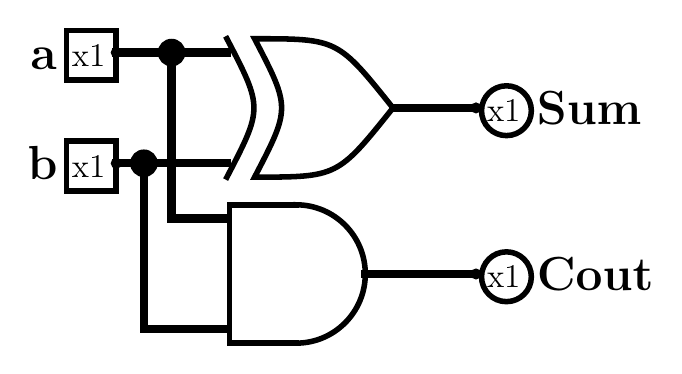
\begin{tikzpicture}[x=1pt,y=-1pt,line cap=rect]
\def\logisimfontA#1{\fontfamily{cmr}{#1}} % Replaced by logisim, original font was "SansSerif"
\definecolor{custcol_0_0_0}{RGB}{0, 0, 0}
\definecolor{custcol_ff_ff_ff}{RGB}{255, 255, 255}
\draw [line width=3.0pt, custcol_0_0_0 ]  (137.0,35.0) -- (167.0,35.0) ;
\draw [line width=3.0pt, custcol_0_0_0 ]  (127.0,95.0) -- (167.0,95.0) ;
\draw [line width=3.0pt, custcol_0_0_0 ]  (37.0,15.0) -- (57.0,15.0) -- (57.0,75.0) -- (77.0,75.0) ;
\draw [line width=3.0pt, custcol_0_0_0 ]  (47.0,55.0) -- (47.0,115.0) -- (77.0,115.0) ;
\fill [line width=3.0pt, custcol_0_0_0]  (47.0,55.0) ellipse (5.0 and 5.0 );
\fill [line width=3.0pt, custcol_0_0_0]  (57.0,15.0) ellipse (5.0 and 5.0 );
\draw [line width=2.0pt, custcol_0_0_0 ]  (19.0,7.0) -- (36.0,7.0) ;
\draw [line width=2.0pt, custcol_0_0_0 ]  (37.0,7.0) -- (37.0,24.0) ;
\draw [line width=2.0pt, custcol_0_0_0 ]  (37.0,25.0) -- (20.0,25.0) ;
\draw [line width=2.0pt, custcol_0_0_0 ]  (19.0,25.0) -- (19.0,8.0) ;
\logisimfontA{\fontsize{12pt}{12pt}\selectfont\node[inner sep=0, outer sep=0, custcol_0_0_0, anchor=base west] at  (21.0,20.0)  {x1};}
\logisimfontA{\fontsize{16pt}{16pt}\fontseries{bx}\selectfont\node[inner sep=0, outer sep=0, custcol_0_0_0, anchor=base west] at  (6.0,21.0)  {a};}
\fill [line width=2.0pt, custcol_0_0_0]  (37.0,15.0) ellipse (2.0 and 2.0 );
\draw [line width=2.0pt, custcol_0_0_0 ]  (19.0,47.0) -- (36.0,47.0) ;
\draw [line width=2.0pt, custcol_0_0_0 ]  (37.0,47.0) -- (37.0,64.0) ;
\draw [line width=2.0pt, custcol_0_0_0 ]  (37.0,65.0) -- (20.0,65.0) ;
\draw [line width=2.0pt, custcol_0_0_0 ]  (19.0,65.0) -- (19.0,48.0) ;
\logisimfontA{\fontsize{12pt}{12pt}\selectfont\node[inner sep=0, outer sep=0, custcol_0_0_0, anchor=base west] at  (21.0,60.0)  {x1};}
\logisimfontA{\fontsize{16pt}{16pt}\fontseries{bx}\selectfont\node[inner sep=0, outer sep=0, custcol_0_0_0, anchor=base west] at  (5.0,61.0)  {b};}
\fill [line width=2.0pt, custcol_0_0_0]  (37.0,55.0) ellipse (2.0 and 2.0 );
\draw [line width=2.0pt, custcol_0_0_0]  (178.0,96.0) ellipse (9.0 and 9.0 );
\logisimfontA{\fontsize{12pt}{12pt}\selectfont\node[inner sep=0, outer sep=0, custcol_0_0_0, anchor=base west] at  (171.0,100.0)  {x1};}
\logisimfontA{\fontsize{16pt}{16pt}\fontseries{bx}\selectfont\node[inner sep=0, outer sep=0, custcol_0_0_0, anchor=base west] at  (189.0,101.0)  {Cout};}
\fill [line width=2.0pt, custcol_0_0_0]  (167.0,95.0) ellipse (2.0 and 2.0 );
\draw [line width=2.0pt, custcol_0_0_0] (102.0,120.0) arc (90.0:-90.0:25.0 and 25.0 );
\draw [line width=2.0pt, custcol_0_0_0 ]  (102.0,70.0) -- (78.0,70.0) -- (78.0,120.0) -- (102.0,120.0) ;
\draw [line width=3.0pt, custcol_0_0_0 ]  (57.0,15.0) -- (77.0,15.0) -- (77.0,15.0) ;
\draw [line width=3.0pt, custcol_0_0_0 ]  (37.0,55.0) -- (47.0,55.0) -- (77.0,55.0) -- (77.0,55.0) ;
\draw [line width=2.0pt, custcol_0_0_0 ]  (137.0,35.0) .. controls  (117.0,10.0)  ..  (87.0,10.0) .. controls  (100.0,35.0)  ..  (87.0,60.0) .. controls  (117.0,60.0)  ..  (137.0,35.0) -- cycle ;
\draw [line width=2.0pt, custcol_0_0_0 ]  (77.0,10.0) .. controls  (90.0,35.0)  ..  (77.0,60.0) ;
\draw [line width=2.0pt, custcol_0_0_0]  (178.0,36.0) ellipse (9.0 and 9.0 );
\logisimfontA{\fontsize{12pt}{12pt}\selectfont\node[inner sep=0, outer sep=0, custcol_0_0_0, anchor=base west] at  (171.0,40.0)  {x1};}
\logisimfontA{\fontsize{16pt}{16pt}\fontseries{bx}\selectfont\node[inner sep=0, outer sep=0, custcol_0_0_0, anchor=base west] at  (189.0,41.0)  {Sum};}
\fill [line width=2.0pt, custcol_0_0_0]  (167.0,35.0) ellipse (2.0 and 2.0 );
\end{tikzpicture}
}

				\label{fig:somadorincompleto}
			\end{figure}
			
		\end{columns}
	}
\end{frame}
\begin{frame}
	\frametitle{Meio somador / Somador incompleto / Half adder}
	\par A tabela-verdade e o circuito mostrados abaixo representam o que chamamos de \textbf{meio somador}, \textbf{somador incompleto} ou ainda \textit{\textbf{Half Adder}}. O meio somador tem essa denominação porque, apesar de realizar a soma de dois bits, não considera um bit que possa vir para complementar sua operação. Dessa forma, o circuito é capaz de trabalhar apenas com a soma de dois bits, informando se houve um bit $C_{out}$. Isso impede a criação de somadores para números maiores por meio da concatenação de vários circuitos
	\begin{columns}
		\column{.5\linewidth}
		\begin{table}[h!]
			\centering
			\begin{tabular}{|c|c|c|c|c|c|}
				\hline
				a & b & Sum & \(C_{out}\)& \(a \oplus b\) & \(a \cdot b\) \\ \hline
				0 & 0 & 0   & 0          & 0              & 0             \\ \hline
				0 & 1 & 1   & 0          & 1              & 0             \\ \hline
				1 & 0 & 1   & 0          & 1              & 0             \\ \hline
				1 & 1 & 0   & 1          & 0              & 1             \\ \hline
			\end{tabular}
			\caption{Tabela verdade da soma binária}
			\label{tab:binary_addition4}
		\end{table}
		\column{.5\linewidth}
		\begin{figure}
			\centering
			% Important: If latex complains about unicode characters,
% please use "\usepackage[utf8x]{inputenc}" in your preamble
% You can change the size of the picture by putting it into the construct:
% 1) \resizebox{10cm}{!}{"below picture"} to scale horizontally to 10 cm
% 2) \resizebox{!}{15cm}{"below picture"} to scale vertically to 15 cm
% 3) \resizebox{10cm}{15cm}{"below picture"} a combination of above two
% It is not recomended to use the scale option of the tikzpicture environment.
\resizebox{\linewidth}{!}{
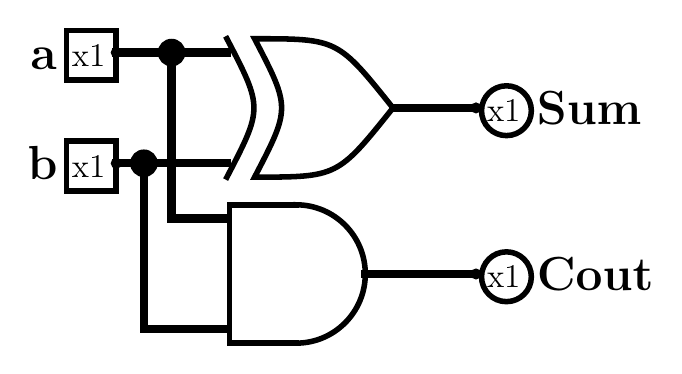
\begin{tikzpicture}[x=1pt,y=-1pt,line cap=rect]
\def\logisimfontA#1{\fontfamily{cmr}{#1}} % Replaced by logisim, original font was "SansSerif"
\definecolor{custcol_0_0_0}{RGB}{0, 0, 0}
\definecolor{custcol_ff_ff_ff}{RGB}{255, 255, 255}
\draw [line width=3.0pt, custcol_0_0_0 ]  (137.0,35.0) -- (167.0,35.0) ;
\draw [line width=3.0pt, custcol_0_0_0 ]  (127.0,95.0) -- (167.0,95.0) ;
\draw [line width=3.0pt, custcol_0_0_0 ]  (37.0,15.0) -- (57.0,15.0) -- (57.0,75.0) -- (77.0,75.0) ;
\draw [line width=3.0pt, custcol_0_0_0 ]  (47.0,55.0) -- (47.0,115.0) -- (77.0,115.0) ;
\fill [line width=3.0pt, custcol_0_0_0]  (47.0,55.0) ellipse (5.0 and 5.0 );
\fill [line width=3.0pt, custcol_0_0_0]  (57.0,15.0) ellipse (5.0 and 5.0 );
\draw [line width=2.0pt, custcol_0_0_0 ]  (19.0,7.0) -- (36.0,7.0) ;
\draw [line width=2.0pt, custcol_0_0_0 ]  (37.0,7.0) -- (37.0,24.0) ;
\draw [line width=2.0pt, custcol_0_0_0 ]  (37.0,25.0) -- (20.0,25.0) ;
\draw [line width=2.0pt, custcol_0_0_0 ]  (19.0,25.0) -- (19.0,8.0) ;
\logisimfontA{\fontsize{12pt}{12pt}\selectfont\node[inner sep=0, outer sep=0, custcol_0_0_0, anchor=base west] at  (21.0,20.0)  {x1};}
\logisimfontA{\fontsize{16pt}{16pt}\fontseries{bx}\selectfont\node[inner sep=0, outer sep=0, custcol_0_0_0, anchor=base west] at  (6.0,21.0)  {a};}
\fill [line width=2.0pt, custcol_0_0_0]  (37.0,15.0) ellipse (2.0 and 2.0 );
\draw [line width=2.0pt, custcol_0_0_0 ]  (19.0,47.0) -- (36.0,47.0) ;
\draw [line width=2.0pt, custcol_0_0_0 ]  (37.0,47.0) -- (37.0,64.0) ;
\draw [line width=2.0pt, custcol_0_0_0 ]  (37.0,65.0) -- (20.0,65.0) ;
\draw [line width=2.0pt, custcol_0_0_0 ]  (19.0,65.0) -- (19.0,48.0) ;
\logisimfontA{\fontsize{12pt}{12pt}\selectfont\node[inner sep=0, outer sep=0, custcol_0_0_0, anchor=base west] at  (21.0,60.0)  {x1};}
\logisimfontA{\fontsize{16pt}{16pt}\fontseries{bx}\selectfont\node[inner sep=0, outer sep=0, custcol_0_0_0, anchor=base west] at  (5.0,61.0)  {b};}
\fill [line width=2.0pt, custcol_0_0_0]  (37.0,55.0) ellipse (2.0 and 2.0 );
\draw [line width=2.0pt, custcol_0_0_0]  (178.0,96.0) ellipse (9.0 and 9.0 );
\logisimfontA{\fontsize{12pt}{12pt}\selectfont\node[inner sep=0, outer sep=0, custcol_0_0_0, anchor=base west] at  (171.0,100.0)  {x1};}
\logisimfontA{\fontsize{16pt}{16pt}\fontseries{bx}\selectfont\node[inner sep=0, outer sep=0, custcol_0_0_0, anchor=base west] at  (189.0,101.0)  {Cout};}
\fill [line width=2.0pt, custcol_0_0_0]  (167.0,95.0) ellipse (2.0 and 2.0 );
\draw [line width=2.0pt, custcol_0_0_0] (102.0,120.0) arc (90.0:-90.0:25.0 and 25.0 );
\draw [line width=2.0pt, custcol_0_0_0 ]  (102.0,70.0) -- (78.0,70.0) -- (78.0,120.0) -- (102.0,120.0) ;
\draw [line width=3.0pt, custcol_0_0_0 ]  (57.0,15.0) -- (77.0,15.0) -- (77.0,15.0) ;
\draw [line width=3.0pt, custcol_0_0_0 ]  (37.0,55.0) -- (47.0,55.0) -- (77.0,55.0) -- (77.0,55.0) ;
\draw [line width=2.0pt, custcol_0_0_0 ]  (137.0,35.0) .. controls  (117.0,10.0)  ..  (87.0,10.0) .. controls  (100.0,35.0)  ..  (87.0,60.0) .. controls  (117.0,60.0)  ..  (137.0,35.0) -- cycle ;
\draw [line width=2.0pt, custcol_0_0_0 ]  (77.0,10.0) .. controls  (90.0,35.0)  ..  (77.0,60.0) ;
\draw [line width=2.0pt, custcol_0_0_0]  (178.0,36.0) ellipse (9.0 and 9.0 );
\logisimfontA{\fontsize{12pt}{12pt}\selectfont\node[inner sep=0, outer sep=0, custcol_0_0_0, anchor=base west] at  (171.0,40.0)  {x1};}
\logisimfontA{\fontsize{16pt}{16pt}\fontseries{bx}\selectfont\node[inner sep=0, outer sep=0, custcol_0_0_0, anchor=base west] at  (189.0,41.0)  {Sum};}
\fill [line width=2.0pt, custcol_0_0_0]  (167.0,35.0) ellipse (2.0 and 2.0 );
\end{tikzpicture}
}

			\label{fig:somadorincompleto2}
		\end{figure}
		
	\end{columns}
\end{frame}
\begin{frame}
	\frametitle{Somador completo}
	\par Para determinar um somador completo, é necessário considerar não apenas as entradas $a$ e $b$, mas também uma entrada $C_{in}$​, que representa o possível bit vindo do $C_{out}$​ de outro circuito. Dessa forma, o resultado da soma é alterado, o que, por sua vez, modifica a expressão final e o circuito resultante.
	\begin{table}[h!]
		\centering
		\begin{tabular}{|c|c|c|c|}
			\hline
			a & b & $C_{in}$ & Sum \\
			\hline
			0 & 0 & 0 & 0 \\
			0 & 0 & 1 & 1 \\
			0 & 1 & 0 & 1 \\
			0 & 1 & 1 & 0 \\
			1 & 0 & 0 & 1 \\
			1 & 0 & 1 & 0 \\
			1 & 1 & 0 & 0 \\
			1 & 1 & 1 & 1 \\
			\hline
		\end{tabular}
		\caption{Tabela verdade de um somador completo}
		\label{tab:full_adder}
	\end{table}
\end{frame}

\begin{frame}
	\frametitle{Somador completo}
	\framesubtitle{\textbf{Prática guiada}}
	\par Considerando a tabela verdade mostrada determine a expressão algébrica boleana e o circuito correspondentes.
	\begin{columns}
		\column{.5\linewidth}
			\begin{table}[h!]
				\centering
				\begin{tabular}{|c|c|c|c|}
					\hline
					a & b & $C_{in}$ & Sum \\
					\hline
					0 & 0 & 0 & 0 \\
					0 & 0 & 1 & 1 \\
					0 & 1 & 0 & 1 \\
					0 & 1 & 1 & 0 \\
					1 & 0 & 0 & 1 \\
					1 & 0 & 1 & 0 \\
					1 & 1 & 0 & 0 \\
					1 & 1 & 1 & 1 \\
					\hline
				\end{tabular}
				\caption{Tabela verdade de $C_{in}$ para somador completo}
				\label{tab:full_adder2}
			\end{table}
		\column{.5\linewidth}
			\pause
			\par Para facilitar a notação considerando $c=C_{in}$ Temos por \textit{mimtermos}:
			\begin{equation}
				\begin{aligned}
					&(\overline{a}\overline{b}c)+(\overline{a}b\overline{c})+(a\overline{b}\overline{c})+(abc) = \\
					&\overline{a}.(\overline{b}c+b\overline{c}) + a.(\overline{b}\overline{c}+bc) = \\
					&\overline{a}.(b \oplus c) + a.(\overline{b \oplus c}) = \\
					& \boxed{a \oplus (b \oplus c)}
				\end{aligned}
			\end{equation}
			\vspace{-0.5cm}
			\pause
			\begin{figure}
				\centering
				% Important: If latex complains about unicode characters,
% please use "\usepackage[utf8x]{inputenc}" in your preamble
% You can change the size of the picture by putting it into the construct:
% 1) \resizebox{10cm}{!}{"below picture"} to scale horizontally to 10 cm
% 2) \resizebox{!}{15cm}{"below picture"} to scale vertically to 15 cm
% 3) \resizebox{10cm}{15cm}{"below picture"} a combination of above two
% It is not recomended to use the scale option of the tikzpicture environment.
\resizebox{!}{1.7cm}{
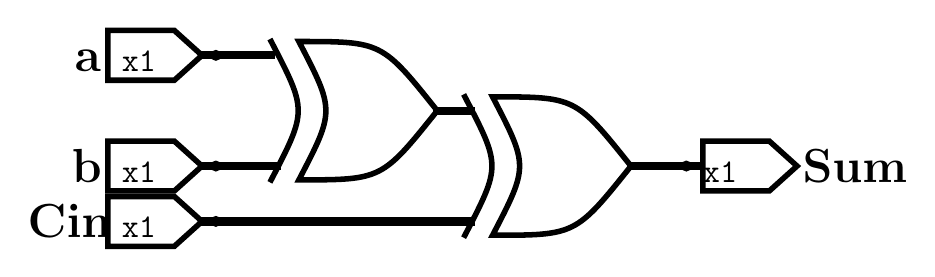
\begin{tikzpicture}[x=1pt,y=-1pt,line cap=rect]
\def\logisimfontA#1{\fontfamily{cmr}{#1}} % Replaced by logisim, original font was "SansSerif"
\def\logisimfontB#1{\fontfamily{cmtt}{#1}} % Replaced by logisim, original font was "Monospaced"
\definecolor{custcol_0_0_0}{RGB}{0, 0, 0}
\definecolor{custcol_ff_ff_ff}{RGB}{255, 255, 255}
\draw [line width=3.0pt, custcol_0_0_0 ]  (223.0,55.0) -- (243.0,55.0) ;
\draw [line width=2.0pt, custcol_0_0_0 ]  (153.0,35.0) .. controls  (133.0,10.0)  ..  (103.0,10.0) .. controls  (116.0,35.0)  ..  (103.0,60.0) .. controls  (133.0,60.0)  ..  (153.0,35.0) -- cycle ;
\draw [line width=2.0pt, custcol_0_0_0 ]  (93.0,10.0) .. controls  (106.0,35.0)  ..  (93.0,60.0) ;
\draw [line width=3.0pt, custcol_0_0_0 ]  (68.0,55.0) -- (73.0,55.0) -- (93.0,55.0) -- (95.0,55.0) ;
\draw [line width=2.0pt, custcol_0_0_0 ]  (58.0,64.0) -- (68.0,55.0) -- (58.0,46.0) -- (34.0,46.0) -- (34.0,64.0) -- cycle;
\logisimfontB{\fontsize{12pt}{12pt}\selectfont\node[inner sep=0, outer sep=0, custcol_0_0_0, anchor=base west] at  (39.0,61.0)  {x1};}
\logisimfontA{\fontsize{16pt}{16pt}\fontseries{bx}\selectfont\node[inner sep=0, outer sep=0, custcol_0_0_0, anchor=base west] at  (21.0,61.0)  {b};}
\fill [line width=2.0pt, custcol_0_0_0]  (73.0,55.0) ellipse (2.0 and 2.0 );
\draw [line width=3.0pt, custcol_0_0_0 ]  (68.0,15.0) -- (73.0,15.0) -- (93.0,15.0) -- (93.0,15.0) ;
\draw [line width=2.0pt, custcol_0_0_0 ]  (58.0,24.0) -- (68.0,15.0) -- (58.0,6.0) -- (34.0,6.0) -- (34.0,24.0) -- cycle;
\logisimfontB{\fontsize{12pt}{12pt}\selectfont\node[inner sep=0, outer sep=0, custcol_0_0_0, anchor=base west] at  (39.0,21.0)  {x1};}
\logisimfontA{\fontsize{16pt}{16pt}\fontseries{bx}\selectfont\node[inner sep=0, outer sep=0, custcol_0_0_0, anchor=base west] at  (22.0,21.0)  {a};}
\fill [line width=2.0pt, custcol_0_0_0]  (73.0,15.0) ellipse (2.0 and 2.0 );
\draw [line width=2.0pt, custcol_0_0_0 ]  (58.0,84.0) -- (68.0,75.0) -- (58.0,66.0) -- (34.0,66.0) -- (34.0,84.0) -- cycle;
\logisimfontB{\fontsize{12pt}{12pt}\selectfont\node[inner sep=0, outer sep=0, custcol_0_0_0, anchor=base west] at  (39.0,81.0)  {x1};}
\logisimfontA{\fontsize{16pt}{16pt}\fontseries{bx}\selectfont\node[inner sep=0, outer sep=0, custcol_0_0_0, anchor=base west] at  (5.0,81.0)  {Cin};}
\fill [line width=2.0pt, custcol_0_0_0]  (73.0,75.0) ellipse (2.0 and 2.0 );
\draw [line width=3.0pt, custcol_0_0_0 ]  (153.0,35.0) -- (163.0,35.0) -- (165.0,35.0) ;
\draw [line width=3.0pt, custcol_0_0_0 ]  (68.0,75.0) -- (73.0,75.0) -- (163.0,75.0) -- (165.0,75.0) ;
\draw [line width=2.0pt, custcol_0_0_0 ]  (223.0,55.0) .. controls  (203.0,30.0)  ..  (173.0,30.0) .. controls  (186.0,55.0)  ..  (173.0,80.0) .. controls  (203.0,80.0)  ..  (223.0,55.0) -- cycle ;
\draw [line width=2.0pt, custcol_0_0_0 ]  (163.0,30.0) .. controls  (176.0,55.0)  ..  (163.0,80.0) ;
\draw [line width=3.0pt, custcol_0_0_0 ]  (247.0,55.0) -- (244.0,55.0) ;
\draw [line width=2.0pt, custcol_0_0_0 ]  (273.0,46.0) -- (283.0,55.0) -- (273.0,64.0) -- (249.0,64.0) -- (249.0,46.0) -- cycle;
\logisimfontB{\fontsize{12pt}{12pt}\selectfont\node[inner sep=0, outer sep=0, custcol_0_0_0, anchor=base west] at  (249.0,61.0)  {x1};}
\logisimfontA{\fontsize{16pt}{16pt}\fontseries{bx}\selectfont\node[inner sep=0, outer sep=0, custcol_0_0_0, anchor=base west] at  (285.0,61.0)  {Sum};}
\fill [line width=2.0pt, custcol_0_0_0]  (243.0,55.0) ellipse (2.0 and 2.0 );
\end{tikzpicture}
}

				\label{fig:somadorcompletoparte01}
			\end{figure}
	\end{columns}
\end{frame}
\begin{frame}
	\frametitle{Somador completo}
	\par Um somador completo deve não apenas receber um $C_{in}$ como também gerar um $C_{out}$. Portanto, é necessário determinar como o $C_{out}$ é obtido.
	\begin{table}[h!]
		\centering
		\begin{tabular}{|c|c|c|c|}
			\hline
			a & b & $C_{in}$ & $C_{out}$ \\
			\hline
			0 & 0 & 0 & \pause 0 \\
			0 & 0 & 1 & \pause 0 \\
			0 & 1 & 0 & \pause 0 \\
			0 & 1 & 1 & \pause 1 \\
			1 & 0 & 0 & \pause 0 \\
			1 & 0 & 1 & \pause 1 \\
			1 & 1 & 0 & \pause 1 \\
			1 & 1 & 1 & \pause 1 \\
			\hline
		\end{tabular}
		\caption{Tabela verdade de $C_{out}$ para somador completo}
		\label{tab:carry_out}
	\end{table}
\end{frame}

\begin{frame}
	\frametitle{Somador completo}
	\framesubtitle{\textbf{Prática dirigida}}
	\par A partir da tabela-verdade mostrada determine a expressão algébrica booleana correspondente e o respectivo circuito de $C_{out}$\footnote[frame]{boa sorte...}.
	
	\begin{columns}
		\column{.6\linewidth}
			\begin{table}[h!]
				\centering
				\begin{tabular}{|c|c|c|c|}
					\hline
					a & b & $C_{in}$ & $C_{out}$ \\
					\hline
					0 & 0 & 0 & 0 \\
					0 & 0 & 1 & 0 \\
					0 & 1 & 0 & 0 \\
					0 & 1 & 1 & 1 \\
					1 & 0 & 0 & 0 \\
					1 & 0 & 1 & 1 \\
					1 & 1 & 0 & 1 \\
					1 & 1 & 1 & 1 \\
					\hline
				\end{tabular}
				\caption{Tabela-verdade de $C_{out}$ para somador completo}
				\label{tab:carry_out2}
			\end{table}
		\column{.4\linewidth}
			\par Para facilitar a notação considerando $c=C_{in}$ temos por \textit{mimtermos}:
			\begin{equation}
				\begin{aligned}
					&(\overline{a}bc)+(a\overline{b}c)+(ab\overline{c})+(abc) = \\
				\end{aligned}
			\end{equation}
	\end{columns}
\end{frame}

\begin{frame}
	\frametitle{Somador completo}
	\framesubtitle{\textbf{Prática dirigida}}
	\begin{columns}
		\column{.5\linewidth}
			\begin{equation}
				\begin{aligned}
					&(\overline{a}bc)+(a\overline{b}c)+(ab\overline{c})+(abc) = \\ \pause
					&\text{reorganizando:} \\
					&(a\overline{b}c)+(ab\overline{c})+(abc)+(\overline{a}bc) = \\ \pause
					&\text{pondo \textbf{a} em evidência:} \\
					&a.(\overline{b}c+b\overline{c}+bc)+(\overline{a}bc) = \\ \pause
					&\text{pondo \textbf{c} em evidência} \\
					&a.(c.(\overline{b}b)+b\overline{c})+(\overline{a}bc) = \\ \pause
					&a.(c.1+b\overline{c})+(\overline{a}bc) = \\ \pause
					&a.(c+b\overline{c})+(\overline{a}bc) = \\ \pause
				\end{aligned}
			\end{equation}
		\column{.5\linewidth}
			\begin{equation}
				\begin{aligned}
					&\text{usando o teorema:} x+\overline{x}y = x+y \\ \pause
					&a.(c+b)+(\overline{a}bc) = \\
					&ac+ab+\overline{a}bc = \\ 
					&\text{colocando \textbf{b} em evidência:} \\ \pause
					&ac+b.(a+\overline{a}c) = \\
					&\text{usando o teorema:} x+\overline{x}y = x+y \\ \pause
					&ac+b.(a+c) = \\
					&\boxed{ac+ba+bc}
				\end{aligned}
			\end{equation}
	\end{columns}
\end{frame}

\begin{frame}
	\frametitle{Somador completo}
	\framesubtitle{\textbf{Prática dirigida}}
	\par Portanto o circuito do $C_{out}$ fica assim:
	\begin{figure}
		\centering
		% Important: If latex complains about unicode characters,
% please use "\usepackage[utf8x]{inputenc}" in your preamble
% You can change the size of the picture by putting it into the construct:
% 1) \resizebox{10cm}{!}{"below picture"} to scale horizontally to 10 cm
% 2) \resizebox{!}{15cm}{"below picture"} to scale vertically to 15 cm
% 3) \resizebox{10cm}{15cm}{"below picture"} a combination of above two
% It is not recomended to use the scale option of the tikzpicture environment.
\resizebox{10cm}{!}{
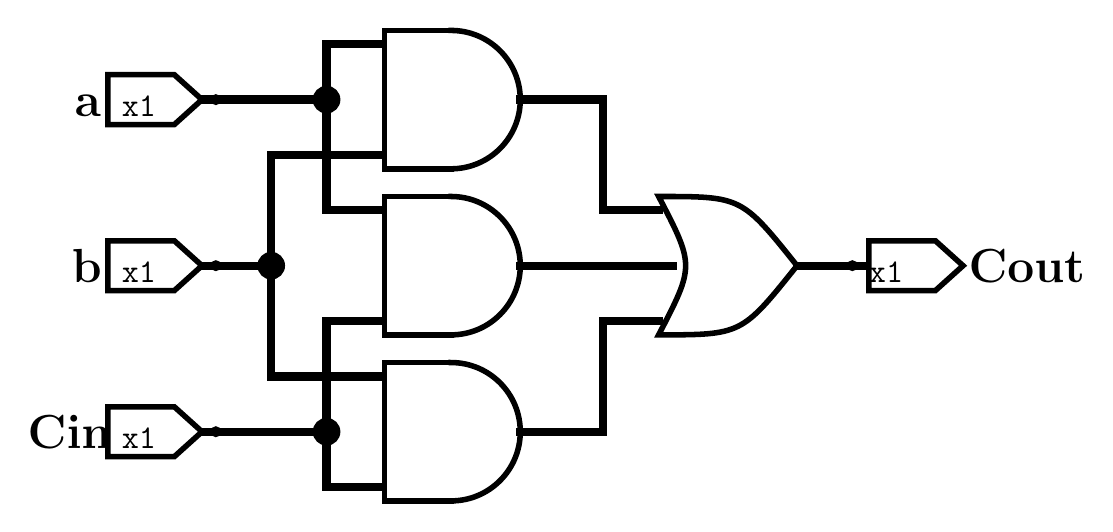
\begin{tikzpicture}[x=1pt,y=-1pt,line cap=rect]
\def\logisimfontA#1{\fontfamily{cmr}{#1}} % Replaced by logisim, original font was "SansSerif"
\def\logisimfontB#1{\fontfamily{cmtt}{#1}} % Replaced by logisim, original font was "Monospaced"
\definecolor{custcol_0_0_0}{RGB}{0, 0, 0}
\definecolor{custcol_ff_ff_ff}{RGB}{255, 255, 255}
\draw [line width=3.0pt, custcol_0_0_0 ]  (283.0,90.0) -- (303.0,90.0) ;
\draw [line width=3.0pt, custcol_0_0_0 ]  (133.0,50.0) -- (93.0,50.0) -- (93.0,90.0) ;
\draw [line width=3.0pt, custcol_0_0_0 ]  (113.0,30.0) -- (113.0,70.0) -- (133.0,70.0) ;
\draw [line width=3.0pt, custcol_0_0_0 ]  (133.0,110.0) -- (113.0,110.0) -- (113.0,150.0) ;
\fill [line width=3.0pt, custcol_0_0_0]  (93.0,90.0) ellipse (5.0 and 5.0 );
\fill [line width=3.0pt, custcol_0_0_0]  (113.0,150.0) ellipse (5.0 and 5.0 );
\fill [line width=3.0pt, custcol_0_0_0]  (113.0,30.0) ellipse (5.0 and 5.0 );
\draw [line width=2.0pt, custcol_0_0_0] (158.0,175.0) arc (90.0:-90.0:25.0 and 25.0 );
\draw [line width=2.0pt, custcol_0_0_0 ]  (158.0,125.0) -- (134.0,125.0) -- (134.0,175.0) -- (158.0,175.0) ;
\draw [line width=2.0pt, custcol_0_0_0] (158.0,115.0) arc (90.0:-90.0:25.0 and 25.0 );
\draw [line width=2.0pt, custcol_0_0_0 ]  (158.0,65.0) -- (134.0,65.0) -- (134.0,115.0) -- (158.0,115.0) ;
\draw [line width=2.0pt, custcol_0_0_0] (158.0,55.0) arc (90.0:-90.0:25.0 and 25.0 );
\draw [line width=2.0pt, custcol_0_0_0 ]  (158.0,5.0) -- (134.0,5.0) -- (134.0,55.0) -- (158.0,55.0) ;
\draw [line width=3.0pt, custcol_0_0_0 ]  (68.0,90.0) -- (73.0,90.0) -- (93.0,90.0) -- (93.0,130.0) -- (133.0,130.0) ;
\draw [line width=2.0pt, custcol_0_0_0 ]  (58.0,99.0) -- (68.0,90.0) -- (58.0,81.0) -- (34.0,81.0) -- (34.0,99.0) -- cycle;
\logisimfontB{\fontsize{12pt}{12pt}\selectfont\node[inner sep=0, outer sep=0, custcol_0_0_0, anchor=base west] at  (39.0,96.0)  {x1};}
\logisimfontA{\fontsize{16pt}{16pt}\fontseries{bx}\selectfont\node[inner sep=0, outer sep=0, custcol_0_0_0, anchor=base west] at  (21.0,96.0)  {b};}
\fill [line width=2.0pt, custcol_0_0_0]  (73.0,90.0) ellipse (2.0 and 2.0 );
\draw [line width=3.0pt, custcol_0_0_0 ]  (68.0,30.0) -- (73.0,30.0) -- (113.0,30.0) -- (113.0,10.0) -- (133.0,10.0) ;
\draw [line width=2.0pt, custcol_0_0_0 ]  (58.0,39.0) -- (68.0,30.0) -- (58.0,21.0) -- (34.0,21.0) -- (34.0,39.0) -- cycle;
\logisimfontB{\fontsize{12pt}{12pt}\selectfont\node[inner sep=0, outer sep=0, custcol_0_0_0, anchor=base west] at  (39.0,36.0)  {x1};}
\logisimfontA{\fontsize{16pt}{16pt}\fontseries{bx}\selectfont\node[inner sep=0, outer sep=0, custcol_0_0_0, anchor=base west] at  (22.0,36.0)  {a};}
\fill [line width=2.0pt, custcol_0_0_0]  (73.0,30.0) ellipse (2.0 and 2.0 );
\draw [line width=3.0pt, custcol_0_0_0 ]  (68.0,150.0) -- (73.0,150.0) -- (113.0,150.0) -- (113.0,170.0) -- (133.0,170.0) ;
\draw [line width=2.0pt, custcol_0_0_0 ]  (58.0,159.0) -- (68.0,150.0) -- (58.0,141.0) -- (34.0,141.0) -- (34.0,159.0) -- cycle;
\logisimfontB{\fontsize{12pt}{12pt}\selectfont\node[inner sep=0, outer sep=0, custcol_0_0_0, anchor=base west] at  (39.0,156.0)  {x1};}
\logisimfontA{\fontsize{16pt}{16pt}\fontseries{bx}\selectfont\node[inner sep=0, outer sep=0, custcol_0_0_0, anchor=base west] at  (5.0,156.0)  {Cin};}
\fill [line width=2.0pt, custcol_0_0_0]  (73.0,150.0) ellipse (2.0 and 2.0 );
\draw [line width=3.0pt, custcol_0_0_0 ]  (183.0,30.0) -- (213.0,30.0) -- (213.0,70.0) -- (233.0,70.0) -- (233.0,70.0) ;
\draw [line width=3.0pt, custcol_0_0_0 ]  (183.0,90.0) -- (233.0,90.0) -- (238.0,90.0) ;
\draw [line width=3.0pt, custcol_0_0_0 ]  (233.0,110.0) -- (233.0,110.0) -- (213.0,110.0) -- (213.0,150.0) -- (183.0,150.0) ;
\draw [line width=2.0pt, custcol_0_0_0 ]  (283.0,90.0) .. controls  (263.0,65.0)  ..  (233.0,65.0) .. controls  (246.0,90.0)  ..  (233.0,115.0) .. controls  (263.0,115.0)  ..  (283.0,90.0) -- cycle ;
\draw [line width=3.0pt, custcol_0_0_0 ]  (307.0,90.0) -- (304.0,90.0) ;
\draw [line width=2.0pt, custcol_0_0_0 ]  (333.0,81.0) -- (343.0,90.0) -- (333.0,99.0) -- (309.0,99.0) -- (309.0,81.0) -- cycle;
\logisimfontB{\fontsize{12pt}{12pt}\selectfont\node[inner sep=0, outer sep=0, custcol_0_0_0, anchor=base west] at  (309.0,96.0)  {x1};}
\logisimfontA{\fontsize{16pt}{16pt}\fontseries{bx}\selectfont\node[inner sep=0, outer sep=0, custcol_0_0_0, anchor=base west] at  (345.0,96.0)  {Cout};}
\fill [line width=2.0pt, custcol_0_0_0]  (303.0,90.0) ellipse (2.0 and 2.0 );
\end{tikzpicture}
}

		\label{fig:somadorcompletoparte02}
	\end{figure}
\end{frame}

\begin{frame}
	\frametitle{Somador completo}
	\framesubtitle{\textbf{Prática dirigida}}
	\par Portanto o circuito \textbf{somador completo} ou \textbf{Full adder} fica assim:
	\begin{figure}
		\centering
		% Important: If latex complains about unicode characters,
% please use "\usepackage[utf8x]{inputenc}" in your preamble
% You can change the size of the picture by putting it into the construct:
% 1) \resizebox{10cm}{!}{"below picture"} to scale horizontally to 10 cm
% 2) \resizebox{!}{15cm}{"below picture"} to scale vertically to 15 cm
% 3) \resizebox{10cm}{15cm}{"below picture"} a combination of above two
% It is not recomended to use the scale option of the tikzpicture environment.
\resizebox{7cm}{!}{
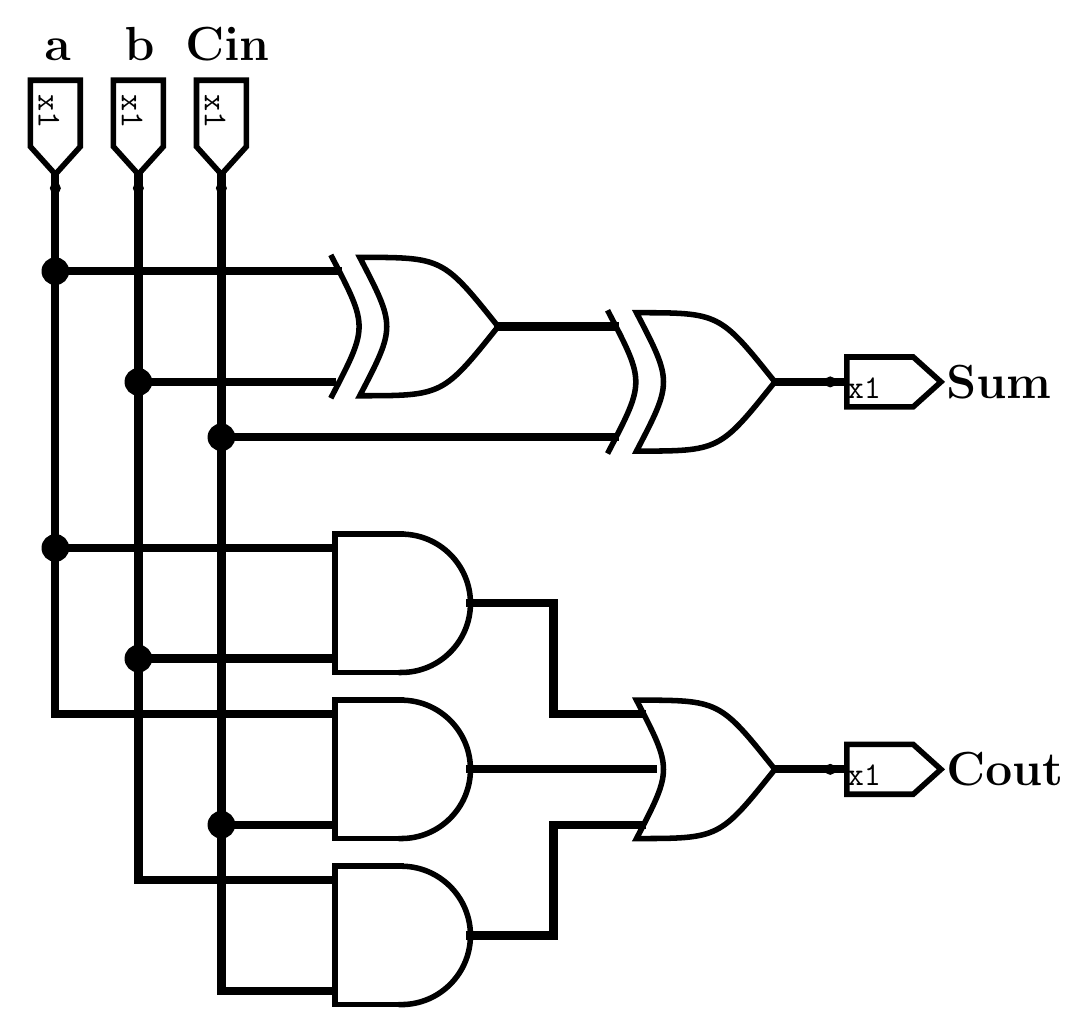
\begin{tikzpicture}[x=1pt,y=-1pt,line cap=rect]
\def\logisimfontA#1{\fontfamily{cmr}{#1}} % Replaced by logisim, original font was "SansSerif"
\def\logisimfontB#1{\fontfamily{cmtt}{#1}} % Replaced by logisim, original font was "Monospaced"
\definecolor{custcol_0_0_0}{RGB}{0, 0, 0}
\definecolor{custcol_ff_ff_ff}{RGB}{255, 255, 255}
\draw [line width=3.0pt, custcol_0_0_0 ]  (15.0,94.0) -- (15.0,194.0) -- (115.0,194.0) ;
\draw [line width=3.0pt, custcol_0_0_0 ]  (275.0,134.0) -- (295.0,134.0) ;
\draw [line width=3.0pt, custcol_0_0_0 ]  (275.0,274.0) -- (295.0,274.0) ;
\draw [line width=3.0pt, custcol_0_0_0 ]  (15.0,194.0) -- (15.0,254.0) -- (115.0,254.0) ;
\draw [line width=3.0pt, custcol_0_0_0 ]  (75.0,294.0) -- (75.0,354.0) -- (115.0,354.0) ;
\draw [line width=3.0pt, custcol_0_0_0 ]  (45.0,234.0) -- (115.0,234.0) ;
\fill [line width=3.0pt, custcol_0_0_0]  (45.0,134.0) ellipse (5.0 and 5.0 );
\fill [line width=3.0pt, custcol_0_0_0]  (15.0,194.0) ellipse (5.0 and 5.0 );
\fill [line width=3.0pt, custcol_0_0_0]  (75.0,154.0) ellipse (5.0 and 5.0 );
\fill [line width=3.0pt, custcol_0_0_0]  (15.0,94.0) ellipse (5.0 and 5.0 );
\fill [line width=3.0pt, custcol_0_0_0]  (75.0,294.0) ellipse (5.0 and 5.0 );
\fill [line width=3.0pt, custcol_0_0_0]  (45.0,234.0) ellipse (5.0 and 5.0 );
\draw [line width=3.0pt, custcol_0_0_0 ]  (75.0,59.0) -- (75.0,64.0) -- (75.0,154.0) -- (75.0,294.0) -- (115.0,294.0) ;
\draw [line width=2.0pt, custcol_0_0_0 ]  (66.0,49.0) -- (75.0,59.0) -- (84.0,49.0) -- (84.0,25.0) -- (66.0,25.0) -- cycle;
\logisimfontB{\fontsize{12pt}{12pt}\selectfont\node[inner sep=0, outer sep=0, custcol_0_0_0, anchor=base west, rotate=-90.0] at  (69.0,30.0)  {x1};}
\logisimfontA{\fontsize{16pt}{16pt}\fontseries{bx}\selectfont\node[inner sep=0, outer sep=0, custcol_0_0_0, anchor=base west] at  (62.0,18.0)  {Cin};}
\fill [line width=2.0pt, custcol_0_0_0]  (75.0,64.0) ellipse (2.0 and 2.0 );
\draw [line width=2.0pt, custcol_0_0_0 ]  (6.0,49.0) -- (15.0,59.0) -- (24.0,49.0) -- (24.0,25.0) -- (6.0,25.0) -- cycle;
\logisimfontB{\fontsize{12pt}{12pt}\selectfont\node[inner sep=0, outer sep=0, custcol_0_0_0, anchor=base west, rotate=-90.0] at  (9.0,30.0)  {x1};}
\logisimfontA{\fontsize{16pt}{16pt}\fontseries{bx}\selectfont\node[inner sep=0, outer sep=0, custcol_0_0_0, anchor=base west] at  (11.0,18.0)  {a};}
\fill [line width=2.0pt, custcol_0_0_0]  (15.0,64.0) ellipse (2.0 and 2.0 );
\draw [line width=2.0pt, custcol_0_0_0] (140.0,359.0) arc (90.0:-90.0:25.0 and 25.0 );
\draw [line width=2.0pt, custcol_0_0_0 ]  (140.0,309.0) -- (116.0,309.0) -- (116.0,359.0) -- (140.0,359.0) ;
\draw [line width=3.0pt, custcol_0_0_0 ]  (165.0,214.0) -- (195.0,214.0) -- (195.0,254.0) -- (225.0,254.0) -- (227.0,254.0) ;
\draw [line width=3.0pt, custcol_0_0_0 ]  (165.0,274.0) -- (225.0,274.0) -- (231.0,274.0) ;
\draw [line width=3.0pt, custcol_0_0_0 ]  (165.0,334.0) -- (195.0,334.0) -- (195.0,294.0) -- (225.0,294.0) -- (227.0,294.0) ;
\draw [line width=2.0pt, custcol_0_0_0 ]  (275.0,274.0) .. controls  (255.0,249.0)  ..  (225.0,249.0) .. controls  (238.0,274.0)  ..  (225.0,299.0) .. controls  (255.0,299.0)  ..  (275.0,274.0) -- cycle ;
\draw [line width=3.0pt, custcol_0_0_0 ]  (175.0,114.0) -- (215.0,114.0) -- (217.0,114.0) ;
\draw [line width=3.0pt, custcol_0_0_0 ]  (75.0,154.0) -- (215.0,154.0) -- (217.0,154.0) ;
\draw [line width=2.0pt, custcol_0_0_0 ]  (275.0,134.0) .. controls  (255.0,109.0)  ..  (225.0,109.0) .. controls  (238.0,134.0)  ..  (225.0,159.0) .. controls  (255.0,159.0)  ..  (275.0,134.0) -- cycle ;
\draw [line width=2.0pt, custcol_0_0_0 ]  (215.0,109.0) .. controls  (228.0,134.0)  ..  (215.0,159.0) ;
\draw [line width=3.0pt, custcol_0_0_0 ]  (299.0,134.0) -- (296.0,134.0) ;
\draw [line width=2.0pt, custcol_0_0_0 ]  (325.0,125.0) -- (335.0,134.0) -- (325.0,143.0) -- (301.0,143.0) -- (301.0,125.0) -- cycle;
\logisimfontB{\fontsize{12pt}{12pt}\selectfont\node[inner sep=0, outer sep=0, custcol_0_0_0, anchor=base west] at  (301.0,140.0)  {x1};}
\logisimfontA{\fontsize{16pt}{16pt}\fontseries{bx}\selectfont\node[inner sep=0, outer sep=0, custcol_0_0_0, anchor=base west] at  (337.0,140.0)  {Sum};}
\fill [line width=2.0pt, custcol_0_0_0]  (295.0,134.0) ellipse (2.0 and 2.0 );
\draw [line width=3.0pt, custcol_0_0_0 ]  (45.0,59.0) -- (45.0,64.0) -- (45.0,134.0) -- (45.0,234.0) -- (45.0,314.0) -- (115.0,314.0) ;
\draw [line width=2.0pt, custcol_0_0_0 ]  (36.0,49.0) -- (45.0,59.0) -- (54.0,49.0) -- (54.0,25.0) -- (36.0,25.0) -- cycle;
\logisimfontB{\fontsize{12pt}{12pt}\selectfont\node[inner sep=0, outer sep=0, custcol_0_0_0, anchor=base west, rotate=-90.0] at  (39.0,30.0)  {x1};}
\logisimfontA{\fontsize{16pt}{16pt}\fontseries{bx}\selectfont\node[inner sep=0, outer sep=0, custcol_0_0_0, anchor=base west] at  (40.0,18.0)  {b};}
\fill [line width=2.0pt, custcol_0_0_0]  (45.0,64.0) ellipse (2.0 and 2.0 );
\draw [line width=2.0pt, custcol_0_0_0] (140.0,299.0) arc (90.0:-90.0:25.0 and 25.0 );
\draw [line width=2.0pt, custcol_0_0_0 ]  (140.0,249.0) -- (116.0,249.0) -- (116.0,299.0) -- (140.0,299.0) ;
\draw [line width=3.0pt, custcol_0_0_0 ]  (299.0,274.0) -- (296.0,274.0) ;
\draw [line width=2.0pt, custcol_0_0_0 ]  (325.0,265.0) -- (335.0,274.0) -- (325.0,283.0) -- (301.0,283.0) -- (301.0,265.0) -- cycle;
\logisimfontB{\fontsize{12pt}{12pt}\selectfont\node[inner sep=0, outer sep=0, custcol_0_0_0, anchor=base west] at  (301.0,280.0)  {x1};}
\logisimfontA{\fontsize{16pt}{16pt}\fontseries{bx}\selectfont\node[inner sep=0, outer sep=0, custcol_0_0_0, anchor=base west] at  (337.0,280.0)  {Cout};}
\fill [line width=2.0pt, custcol_0_0_0]  (295.0,274.0) ellipse (2.0 and 2.0 );
\draw [line width=2.0pt, custcol_0_0_0] (140.0,239.0) arc (90.0:-90.0:25.0 and 25.0 );
\draw [line width=2.0pt, custcol_0_0_0 ]  (140.0,189.0) -- (116.0,189.0) -- (116.0,239.0) -- (140.0,239.0) ;
\draw [line width=3.0pt, custcol_0_0_0 ]  (15.0,59.0) -- (15.0,64.0) -- (15.0,94.0) -- (115.0,94.0) -- (117.0,94.0) ;
\draw [line width=3.0pt, custcol_0_0_0 ]  (45.0,134.0) -- (115.0,134.0) -- (115.0,134.0) ;
\draw [line width=2.0pt, custcol_0_0_0 ]  (175.0,114.0) .. controls  (155.0,89.0)  ..  (125.0,89.0) .. controls  (138.0,114.0)  ..  (125.0,139.0) .. controls  (155.0,139.0)  ..  (175.0,114.0) -- cycle ;
\draw [line width=2.0pt, custcol_0_0_0 ]  (115.0,89.0) .. controls  (128.0,114.0)  ..  (115.0,139.0) ;
\end{tikzpicture}
}

		\label{fig:somadorcompleto}
	\end{figure}
\end{frame}

\begin{frame}
	\frametitle{Somador completo - Gambiarra}
	\par Usando somadores incompletos podemos fazer um completo:
	\begin{figure}
		\centering
		% Important: If latex complains about unicode characters,
% please use "\usepackage[utf8x]{inputenc}" in your preamble
% You can change the size of the picture by putting it into the construct:
% 1) \resizebox{10cm}{!}{"below picture"} to scale horizontally to 10 cm
% 2) \resizebox{!}{15cm}{"below picture"} to scale vertically to 15 cm
% 3) \resizebox{10cm}{15cm}{"below picture"} a combination of above two
% It is not recomended to use the scale option of the tikzpicture environment.
\resizebox{15cm}{!}{
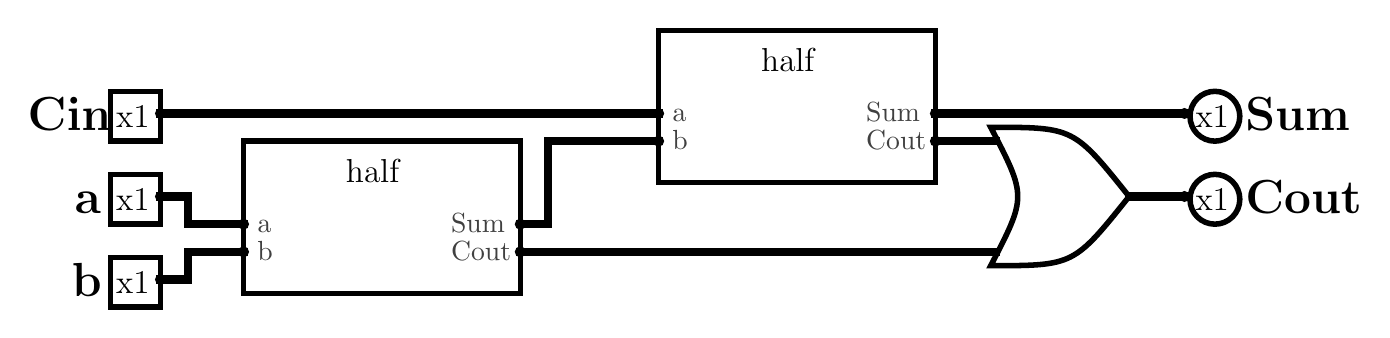
\begin{tikzpicture}[x=1pt,y=-1pt,line cap=rect]
\def\logisimfontA#1{\fontfamily{cmr}{#1}} % Replaced by logisim, original font was "SansSerif"
\definecolor{custcol_0_0_0}{RGB}{0, 0, 0}
\definecolor{custcol_40_40_40}{RGB}{64, 64, 64}
\definecolor{custcol_ff_ff_ff}{RGB}{255, 255, 255}
\draw [line width=3.0pt, custcol_0_0_0 ]  (333.0,36.0) -- (423.0,36.0) ;
\draw [line width=3.0pt, custcol_0_0_0 ]  (403.0,66.0) -- (423.0,66.0) ;
\draw [line width=3.0pt, custcol_0_0_0 ]  (53.0,36.0) -- (233.0,36.0) ;
\draw [line width=3.0pt, custcol_0_0_0 ]  (53.0,66.0) -- (63.0,66.0) -- (63.0,76.0) -- (83.0,76.0) ;
\draw [line width=3.0pt, custcol_0_0_0 ]  (53.0,96.0) -- (63.0,96.0) -- (63.0,86.0) -- (83.0,86.0) ;
\draw [line width=3.0pt, custcol_0_0_0 ]  (183.0,76.0) -- (193.0,76.0) -- (193.0,46.0) -- (233.0,46.0) ;
\draw [line width=2.0pt, custcol_0_0_0 ]  (233.0,6.0) -- (332.0,6.0) ;
\draw [line width=2.0pt, custcol_0_0_0 ]  (333.0,6.0) -- (333.0,60.0) ;
\draw [line width=2.0pt, custcol_0_0_0 ]  (333.0,61.0) -- (234.0,61.0) ;
\draw [line width=2.0pt, custcol_0_0_0 ]  (233.0,61.0) -- (233.0,7.0) ;
\logisimfontA{\fontsize{10pt}{10pt}\selectfont\node[inner sep=0, outer sep=0, custcol_40_40_40, anchor=base west] at  (238.0,39.0)  {a};}
\logisimfontA{\fontsize{10pt}{10pt}\selectfont\node[inner sep=0, outer sep=0, custcol_40_40_40, anchor=base west] at  (238.0,49.0)  {b};}
\logisimfontA{\fontsize{10pt}{10pt}\selectfont\node[inner sep=0, outer sep=0, custcol_40_40_40, anchor=base west] at  (308.0,39.0)  {Sum};}
\logisimfontA{\fontsize{10pt}{10pt}\selectfont\node[inner sep=0, outer sep=0, custcol_40_40_40, anchor=base west] at  (308.0,49.0)  {Cout};}
\logisimfontA{\fontsize{12pt}{12pt}\selectfont\node[inner sep=0, outer sep=0, custcol_0_0_0, anchor=base west] at  (270.0,21.0)  {half};}
\fill [line width=1.0pt, custcol_0_0_0]  (233.0,36.0) ellipse (2.0 and 2.0 );
\fill [line width=1.0pt, custcol_0_0_0]  (233.0,46.0) ellipse (2.0 and 2.0 );
\fill [line width=1.0pt, custcol_0_0_0]  (333.0,36.0) ellipse (2.0 and 2.0 );
\fill [line width=1.0pt, custcol_0_0_0]  (333.0,46.0) ellipse (2.0 and 2.0 );
\draw [line width=2.0pt, custcol_0_0_0 ]  (83.0,46.0) -- (182.0,46.0) ;
\draw [line width=2.0pt, custcol_0_0_0 ]  (183.0,46.0) -- (183.0,100.0) ;
\draw [line width=2.0pt, custcol_0_0_0 ]  (183.0,101.0) -- (84.0,101.0) ;
\draw [line width=2.0pt, custcol_0_0_0 ]  (83.0,101.0) -- (83.0,47.0) ;
\logisimfontA{\fontsize{10pt}{10pt}\selectfont\node[inner sep=0, outer sep=0, custcol_40_40_40, anchor=base west] at  (88.0,79.0)  {a};}
\logisimfontA{\fontsize{10pt}{10pt}\selectfont\node[inner sep=0, outer sep=0, custcol_40_40_40, anchor=base west] at  (88.0,89.0)  {b};}
\logisimfontA{\fontsize{10pt}{10pt}\selectfont\node[inner sep=0, outer sep=0, custcol_40_40_40, anchor=base west] at  (158.0,79.0)  {Sum};}
\logisimfontA{\fontsize{10pt}{10pt}\selectfont\node[inner sep=0, outer sep=0, custcol_40_40_40, anchor=base west] at  (158.0,89.0)  {Cout};}
\logisimfontA{\fontsize{12pt}{12pt}\selectfont\node[inner sep=0, outer sep=0, custcol_0_0_0, anchor=base west] at  (120.0,61.0)  {half};}
\fill [line width=1.0pt, custcol_0_0_0]  (83.0,76.0) ellipse (2.0 and 2.0 );
\fill [line width=1.0pt, custcol_0_0_0]  (83.0,86.0) ellipse (2.0 and 2.0 );
\fill [line width=1.0pt, custcol_0_0_0]  (183.0,76.0) ellipse (2.0 and 2.0 );
\fill [line width=1.0pt, custcol_0_0_0]  (183.0,86.0) ellipse (2.0 and 2.0 );
\draw [line width=2.0pt, custcol_0_0_0 ]  (35.0,28.0) -- (52.0,28.0) ;
\draw [line width=2.0pt, custcol_0_0_0 ]  (53.0,28.0) -- (53.0,45.0) ;
\draw [line width=2.0pt, custcol_0_0_0 ]  (53.0,46.0) -- (36.0,46.0) ;
\draw [line width=2.0pt, custcol_0_0_0 ]  (35.0,46.0) -- (35.0,29.0) ;
\logisimfontA{\fontsize{12pt}{12pt}\selectfont\node[inner sep=0, outer sep=0, custcol_0_0_0, anchor=base west] at  (37.0,41.0)  {x1};}
\logisimfontA{\fontsize{16pt}{16pt}\fontseries{bx}\selectfont\node[inner sep=0, outer sep=0, custcol_0_0_0, anchor=base west] at  (5.0,42.0)  {Cin};}
\fill [line width=2.0pt, custcol_0_0_0]  (53.0,36.0) ellipse (2.0 and 2.0 );
\draw [line width=2.0pt, custcol_0_0_0 ]  (35.0,58.0) -- (52.0,58.0) ;
\draw [line width=2.0pt, custcol_0_0_0 ]  (53.0,58.0) -- (53.0,75.0) ;
\draw [line width=2.0pt, custcol_0_0_0 ]  (53.0,76.0) -- (36.0,76.0) ;
\draw [line width=2.0pt, custcol_0_0_0 ]  (35.0,76.0) -- (35.0,59.0) ;
\logisimfontA{\fontsize{12pt}{12pt}\selectfont\node[inner sep=0, outer sep=0, custcol_0_0_0, anchor=base west] at  (37.0,71.0)  {x1};}
\logisimfontA{\fontsize{16pt}{16pt}\fontseries{bx}\selectfont\node[inner sep=0, outer sep=0, custcol_0_0_0, anchor=base west] at  (22.0,72.0)  {a};}
\fill [line width=2.0pt, custcol_0_0_0]  (53.0,66.0) ellipse (2.0 and 2.0 );
\draw [line width=2.0pt, custcol_0_0_0 ]  (35.0,88.0) -- (52.0,88.0) ;
\draw [line width=2.0pt, custcol_0_0_0 ]  (53.0,88.0) -- (53.0,105.0) ;
\draw [line width=2.0pt, custcol_0_0_0 ]  (53.0,106.0) -- (36.0,106.0) ;
\draw [line width=2.0pt, custcol_0_0_0 ]  (35.0,106.0) -- (35.0,89.0) ;
\logisimfontA{\fontsize{12pt}{12pt}\selectfont\node[inner sep=0, outer sep=0, custcol_0_0_0, anchor=base west] at  (37.0,101.0)  {x1};}
\logisimfontA{\fontsize{16pt}{16pt}\fontseries{bx}\selectfont\node[inner sep=0, outer sep=0, custcol_0_0_0, anchor=base west] at  (21.0,102.0)  {b};}
\fill [line width=2.0pt, custcol_0_0_0]  (53.0,96.0) ellipse (2.0 and 2.0 );
\draw [line width=3.0pt, custcol_0_0_0 ]  (333.0,46.0) -- (353.0,46.0) -- (355.0,46.0) ;
\draw [line width=3.0pt, custcol_0_0_0 ]  (183.0,86.0) -- (353.0,86.0) -- (355.0,86.0) ;
\draw [line width=2.0pt, custcol_0_0_0 ]  (403.0,66.0) .. controls  (383.0,41.0)  ..  (353.0,41.0) .. controls  (366.0,66.0)  ..  (353.0,91.0) .. controls  (383.0,91.0)  ..  (403.0,66.0) -- cycle ;
\draw [line width=2.0pt, custcol_0_0_0]  (434.0,67.0) ellipse (9.0 and 9.0 );
\logisimfontA{\fontsize{12pt}{12pt}\selectfont\node[inner sep=0, outer sep=0, custcol_0_0_0, anchor=base west] at  (427.0,71.0)  {x1};}
\logisimfontA{\fontsize{16pt}{16pt}\fontseries{bx}\selectfont\node[inner sep=0, outer sep=0, custcol_0_0_0, anchor=base west] at  (445.0,72.0)  {Cout};}
\fill [line width=2.0pt, custcol_0_0_0]  (423.0,66.0) ellipse (2.0 and 2.0 );
\draw [line width=2.0pt, custcol_0_0_0]  (434.0,37.0) ellipse (9.0 and 9.0 );
\logisimfontA{\fontsize{12pt}{12pt}\selectfont\node[inner sep=0, outer sep=0, custcol_0_0_0, anchor=base west] at  (427.0,41.0)  {x1};}
\logisimfontA{\fontsize{16pt}{16pt}\fontseries{bx}\selectfont\node[inner sep=0, outer sep=0, custcol_0_0_0, anchor=base west] at  (445.0,42.0)  {Sum};}
\fill [line width=2.0pt, custcol_0_0_0]  (423.0,36.0) ellipse (2.0 and 2.0 );
\end{tikzpicture}
}

		\label{fig:somadorcompletogambiarra}
	\end{figure}
\end{frame}

\subsection{Subtratores}

\begin{frame}
	\frametitle{Subtração binária}
	\framesubtitle{Expressão de exemplo}
	\par Abaixo foi realizada uma operação de subtração simples entre dois números binários, a e b, cujo resultado é mostrado na linha marcada com a palavra 'Diff'. '$B_{out}$' significa 'Borrow out', o nosso famoso 'emprestar'. A partir deste exemplo, vamos criar uma tabela-verdade que nos permitirá formular a expressão algébrica booleana e, consequentemente, o circuito subtrator correspondente.
	\begin{table}[h!]
		\centering
		\begin{tabular}{cccc>{\centering\arraybackslash}p{2cm}}
			& 10 & 10 & 10 & $B_{out}$ \\
			1 & 1 & 0 & 0 & $a$\\
			& 1 & 1 & 1 & $b$ \\
			\hline
			& 1 & 0 & 1 & $Diff$ \\
		\end{tabular}
	\end{table}
\end{frame}

\begin{frame}
	\frametitle{Meio subtrator / Subtrator incompleto / Half subtractor}
	\par A tabela-verdade e o circuito mostrados abaixo representam o que chamamos de \textbf{meio subtrator}, \textbf{subtrator incompleto} ou ainda \textit{\textbf{Half subtrator}}. O meio subtrator tem essa denominação porque, apesar de realizar a subtração de dois bits, não considera um bit que possa ter sido emprestado por uma operação de subtração anterior. Dessa forma, o circuito é capaz de trabalhar apenas com a subtração de dois bits, informando se houve necessidade de empréstimo de um bit $B_{out}$. Isso impede a criação de subtratores para números maiores por meio da concatenação de vários circuitos
	\begin{table}[h!]
		\centering
		\begin{tabular}{|c|c|c|c|}
			\hline
			a & b & Diff & \(B_{out}\) \\ \hline
			0 & 0 & 0   & 0          \\ \hline
			0 & 1 & 1   & 1          \\ \hline
			1 & 0 & 1   & 0          \\ \hline
			1 & 1 & 0   & 0          \\ \hline
		\end{tabular}
		\caption{Tabela verdade da diferença binária}
		\label{tab:binary_subtraction}
	\end{table}
\end{frame}

\begin{frame}
	\frametitle{Meio subtrator / Subtrator incompleto / Half subtractor}
	\framesubtitle{\textbf{Prática dirigida} - Tabela verdade da subtração}
	\par Como $Diff$ e $B_{out}$ se comportam? Qual o circuito correspondente?
	\begin{table}[h!]
		\centering
		\begin{tabular}{|c|c|c|c|}
			\hline
			a & b & Diff & \(B_{out}\) \\ \hline
			0 & 0 & 0   & 0          \\ \hline
			0 & 1 & 1   & 1          \\ \hline
			1 & 0 & 1   & 0          \\ \hline
			1 & 1 & 0   & 0          \\ \hline
		\end{tabular}
		\caption{Tabela verdade da diferença binária}
		\label{tab:binary_subtraction2}
	\end{table}
\end{frame}

\begin{frame}
	\frametitle{Meio subtrator / Subtrator incompleto / Half subtractor}
	\framesubtitle{\textbf{Prática dirigida} - Tabela verdade da subtração}
	\begin{columns}
		\column{.5\linewidth}
		\begin{table}[h!]
			\centering
			\begin{tabular}{|c|c|c|c|c|c|}
				\hline
				a & b & Diff & \(B_{out}\)& \(a \oplus b\) & \(\overline{a}.b\) \\ \hline
				0 & 0 & 0   & 0          & 0              & 0             \\ \hline
				0 & 1 & 1   & 1          & 1              & 1             \\ \hline
				1 & 0 & 1   & 0          & 1              & 0             \\ \hline
				1 & 1 & 0   & 0          & 0              & 0             \\ \hline
			\end{tabular}
			\caption{Tabela verdade da diferença binária}
			\label{tab:binary_subtraction3}
		\end{table}
		\pause
		\column{.5\linewidth}
		\begin{figure}
			\centering
			% Important: If latex complains about unicode characters,
% please use "\usepackage[utf8x]{inputenc}" in your preamble
% You can change the size of the picture by putting it into the construct:
% 1) \resizebox{10cm}{!}{"below picture"} to scale horizontally to 10 cm
% 2) \resizebox{!}{15cm}{"below picture"} to scale vertically to 15 cm
% 3) \resizebox{10cm}{15cm}{"below picture"} a combination of above two
% It is not recomended to use the scale option of the tikzpicture environment.
\resizebox{6cm}{!}{
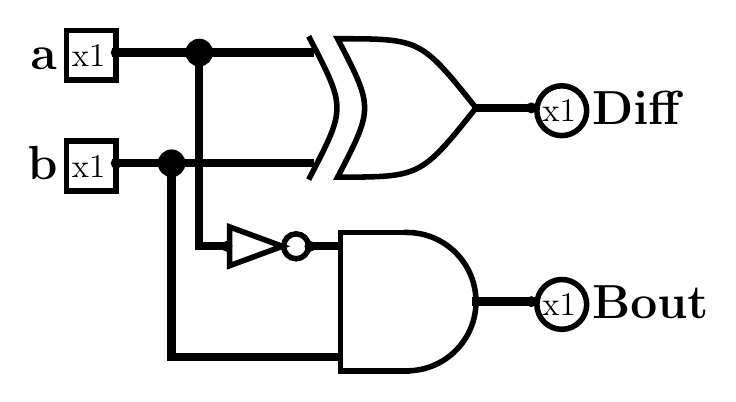
\begin{tikzpicture}[x=1pt,y=-1pt,line cap=rect]
\def\logisimfontA#1{\fontfamily{cmr}{#1}} % Replaced by logisim, original font was "SansSerif"
\definecolor{custcol_0_0_0}{RGB}{0, 0, 0}
\definecolor{custcol_ff_ff_ff}{RGB}{255, 255, 255}
\draw [line width=3.0pt, custcol_0_0_0 ]  (37.0,15.0) -- (67.0,15.0) -- (67.0,85.0) -- (77.0,85.0) ;
\draw [line width=3.0pt, custcol_0_0_0 ]  (107.0,85.0) -- (117.0,85.0) ;
\draw [line width=3.0pt, custcol_0_0_0 ]  (167.0,35.0) -- (187.0,35.0) ;
\draw [line width=3.0pt, custcol_0_0_0 ]  (167.0,105.0) -- (187.0,105.0) ;
\draw [line width=3.0pt, custcol_0_0_0 ]  (37.0,55.0) -- (57.0,55.0) ;
\fill [line width=3.0pt, custcol_0_0_0]  (57.0,55.0) ellipse (5.0 and 5.0 );
\fill [line width=3.0pt, custcol_0_0_0]  (67.0,15.0) ellipse (5.0 and 5.0 );
\draw [line width=2.0pt, custcol_0_0_0 ]  (19.0,7.0) -- (36.0,7.0) ;
\draw [line width=2.0pt, custcol_0_0_0 ]  (37.0,7.0) -- (37.0,24.0) ;
\draw [line width=2.0pt, custcol_0_0_0 ]  (37.0,25.0) -- (20.0,25.0) ;
\draw [line width=2.0pt, custcol_0_0_0 ]  (19.0,25.0) -- (19.0,8.0) ;
\logisimfontA{\fontsize{12pt}{12pt}\selectfont\node[inner sep=0, outer sep=0, custcol_0_0_0, anchor=base west] at  (21.0,20.0)  {x1};}
\logisimfontA{\fontsize{16pt}{16pt}\fontseries{bx}\selectfont\node[inner sep=0, outer sep=0, custcol_0_0_0, anchor=base west] at  (6.0,21.0)  {a};}
\fill [line width=2.0pt, custcol_0_0_0]  (37.0,15.0) ellipse (2.0 and 2.0 );
\draw [line width=2.0pt, custcol_0_0_0 ]  (19.0,47.0) -- (36.0,47.0) ;
\draw [line width=2.0pt, custcol_0_0_0 ]  (37.0,47.0) -- (37.0,64.0) ;
\draw [line width=2.0pt, custcol_0_0_0 ]  (37.0,65.0) -- (20.0,65.0) ;
\draw [line width=2.0pt, custcol_0_0_0 ]  (19.0,65.0) -- (19.0,48.0) ;
\logisimfontA{\fontsize{12pt}{12pt}\selectfont\node[inner sep=0, outer sep=0, custcol_0_0_0, anchor=base west] at  (21.0,60.0)  {x1};}
\logisimfontA{\fontsize{16pt}{16pt}\fontseries{bx}\selectfont\node[inner sep=0, outer sep=0, custcol_0_0_0, anchor=base west] at  (5.0,61.0)  {b};}
\fill [line width=2.0pt, custcol_0_0_0]  (37.0,55.0) ellipse (2.0 and 2.0 );
\draw [line width=3.0pt, custcol_0_0_0 ]  (67.0,15.0) -- (107.0,15.0) -- (107.0,15.0) ;
\draw [line width=3.0pt, custcol_0_0_0 ]  (117.0,125.0) -- (57.0,125.0) -- (57.0,55.0) -- (107.0,55.0) -- (107.0,55.0) ;
\draw [line width=2.0pt, custcol_0_0_0 ]  (167.0,35.0) .. controls  (147.0,10.0)  ..  (117.0,10.0) .. controls  (130.0,35.0)  ..  (117.0,60.0) .. controls  (147.0,60.0)  ..  (167.0,35.0) -- cycle ;
\draw [line width=2.0pt, custcol_0_0_0 ]  (107.0,10.0) .. controls  (120.0,35.0)  ..  (107.0,60.0) ;
\draw [line width=2.0pt, custcol_0_0_0]  (198.0,36.0) ellipse (9.0 and 9.0 );
\logisimfontA{\fontsize{12pt}{12pt}\selectfont\node[inner sep=0, outer sep=0, custcol_0_0_0, anchor=base west] at  (191.0,40.0)  {x1};}
\logisimfontA{\fontsize{16pt}{16pt}\fontseries{bx}\selectfont\node[inner sep=0, outer sep=0, custcol_0_0_0, anchor=base west] at  (209.0,41.0)  {Diff};}
\fill [line width=2.0pt, custcol_0_0_0]  (187.0,35.0) ellipse (2.0 and 2.0 );
\draw [line width=2.0pt, custcol_0_0_0 ]  (97.0,85.0) -- (78.0,78.0) -- (78.0,92.0) -- cycle;
\draw [line width=2.0pt, custcol_0_0_0]  (102.0,85.0) ellipse (4.5 and 4.5 );
\fill [line width=2.0pt, custcol_0_0_0]  (107.0,85.0) ellipse (2.0 and 2.0 );
\fill [line width=2.0pt, custcol_0_0_0]  (77.0,85.0) ellipse (2.0 and 2.0 );
\draw [line width=2.0pt, custcol_0_0_0]  (198.0,106.0) ellipse (9.0 and 9.0 );
\logisimfontA{\fontsize{12pt}{12pt}\selectfont\node[inner sep=0, outer sep=0, custcol_0_0_0, anchor=base west] at  (191.0,110.0)  {x1};}
\logisimfontA{\fontsize{16pt}{16pt}\fontseries{bx}\selectfont\node[inner sep=0, outer sep=0, custcol_0_0_0, anchor=base west] at  (209.0,111.0)  {Bout};}
\fill [line width=2.0pt, custcol_0_0_0]  (187.0,105.0) ellipse (2.0 and 2.0 );
\draw [line width=2.0pt, custcol_0_0_0] (142.0,130.0) arc (90.0:-90.0:25.0 and 25.0 );
\draw [line width=2.0pt, custcol_0_0_0 ]  (142.0,80.0) -- (118.0,80.0) -- (118.0,130.0) -- (142.0,130.0) ;
\end{tikzpicture}
}

			\label{fig:subtratorimcompleto}
		\end{figure}
	\end{columns}
\end{frame}



























\begin{frame}
	\frametitle{Subtrator completo}
	\par Para determinar um subtrator completo, é necessário considerar não apenas as entradas $a$ e $b$, mas também uma entrada $B_{in}$​, que representa o possível bit subtrator vindo do $B_{out}$​ de outro circuito. Dessa forma, o resultado da subtração é alterado, o que, por sua vez, modifica a expressão final e o circuito resultante.
	\par Tenha em mente que $Diff = a-b-B_{in}$.
	\begin{table}[h!]
		\centering
		\begin{tabular}{|c|c|c|c|c|}
			\hline
			a & b & $B_{in}$ & Diff & $B_{out}$ \\
			\hline
			0 & 0 & 0 & 0 & 0 \\
			0 & 0 & 1 & 1 & 1 \\
			0 & 1 & 0 & 1 & 1 \\
			0 & 1 & 1 & 0 & 1 \\
			1 & 0 & 0 & 1 & 0 \\
			1 & 0 & 1 & 0 & 0 \\
			1 & 1 & 0 & 0 & 0 \\
			1 & 1 & 1 & 1 & 1 \\
			\hline
		\end{tabular}
		\caption{Tabela verdade de um subtrator completo}
		\label{tab:full_subtractor}
	\end{table}
\end{frame}

\begin{frame}
	\frametitle{Subtrator completo}
	\framesubtitle{\textbf{Prática guiada}}
	\par Considerando a tabela verdade mostrada determine as expressões algébricas boleanas e os circuitos de $Diff$ e $B_{out}$ correspondentes.
	\begin{columns}
		\column{.5\linewidth}
		\begin{table}[h!]
			\centering
			\begin{tabular}{|c|c|c|c|c|}
				\hline
				a & b & $B_{in}$ & Diff & $B_{out}$ \\
				\hline
				0 & 0 & 0 & 0 & 0 \\
				0 & 0 & 1 & 1 & 1 \\
				0 & 1 & 0 & 1 & 1 \\
				0 & 1 & 1 & 0 & 1 \\
				1 & 0 & 0 & 1 & 0 \\
				1 & 0 & 1 & 0 & 0 \\
				1 & 1 & 0 & 0 & 0 \\
				1 & 1 & 1 & 1 & 1 \\
				\hline
			\end{tabular}
			\caption{Tabela verdade de $B_{in}$ para subtrator completo}
			\label{tab:full_subtractor2}
		\end{table}
		\column{.5\linewidth}
		\pause
		\par Se você olhou bem, economizou tempo! Pois $Diff = a \oplus b \oplus c \therefore$ $\boxed{Diff=a \oplus b \oplus B_{in}}$
		\pause
		\begin{figure}
			\centering
			% Important: If latex complains about unicode characters,
% please use "\usepackage[utf8x]{inputenc}" in your preamble
% You can change the size of the picture by putting it into the construct:
% 1) \resizebox{10cm}{!}{"below picture"} to scale horizontally to 10 cm
% 2) \resizebox{!}{15cm}{"below picture"} to scale vertically to 15 cm
% 3) \resizebox{10cm}{15cm}{"below picture"} a combination of above two
% It is not recomended to use the scale option of the tikzpicture environment.
\resizebox{7cm}{!}{
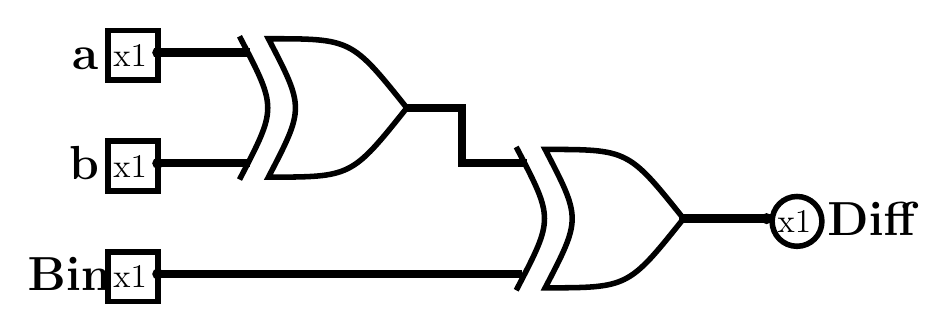
\begin{tikzpicture}[x=1pt,y=-1pt,line cap=rect]
\def\logisimfontA#1{\fontfamily{cmr}{#1}} % Replaced by logisim, original font was "SansSerif"
\definecolor{custcol_0_0_0}{RGB}{0, 0, 0}
\definecolor{custcol_ff_ff_ff}{RGB}{255, 255, 255}
\draw [line width=3.0pt, custcol_0_0_0 ]  (242.0,75.0) -- (272.0,75.0) ;
\draw [line width=3.0pt, custcol_0_0_0 ]  (52.0,15.0) -- (82.0,15.0) -- (84.0,15.0) ;
\draw [line width=3.0pt, custcol_0_0_0 ]  (52.0,55.0) -- (82.0,55.0) -- (84.0,55.0) ;
\draw [line width=2.0pt, custcol_0_0_0 ]  (142.0,35.0) .. controls  (122.0,10.0)  ..  (92.0,10.0) .. controls  (105.0,35.0)  ..  (92.0,60.0) .. controls  (122.0,60.0)  ..  (142.0,35.0) -- cycle ;
\draw [line width=2.0pt, custcol_0_0_0 ]  (82.0,10.0) .. controls  (95.0,35.0)  ..  (82.0,60.0) ;
\draw [line width=2.0pt, custcol_0_0_0]  (283.0,76.0) ellipse (9.0 and 9.0 );
\logisimfontA{\fontsize{12pt}{12pt}\selectfont\node[inner sep=0, outer sep=0, custcol_0_0_0, anchor=base west] at  (276.0,80.0)  {x1};}
\logisimfontA{\fontsize{16pt}{16pt}\fontseries{bx}\selectfont\node[inner sep=0, outer sep=0, custcol_0_0_0, anchor=base west] at  (294.0,81.0)  {Diff};}
\fill [line width=2.0pt, custcol_0_0_0]  (272.0,75.0) ellipse (2.0 and 2.0 );
\draw [line width=3.0pt, custcol_0_0_0 ]  (142.0,35.0) -- (162.0,35.0) -- (162.0,55.0) -- (182.0,55.0) -- (184.0,55.0) ;
\draw [line width=3.0pt, custcol_0_0_0 ]  (52.0,95.0) -- (182.0,95.0) -- (182.0,95.0) ;
\draw [line width=2.0pt, custcol_0_0_0 ]  (242.0,75.0) .. controls  (222.0,50.0)  ..  (192.0,50.0) .. controls  (205.0,75.0)  ..  (192.0,100.0) .. controls  (222.0,100.0)  ..  (242.0,75.0) -- cycle ;
\draw [line width=2.0pt, custcol_0_0_0 ]  (182.0,50.0) .. controls  (195.0,75.0)  ..  (182.0,100.0) ;
\draw [line width=2.0pt, custcol_0_0_0 ]  (34.0,7.0) -- (51.0,7.0) ;
\draw [line width=2.0pt, custcol_0_0_0 ]  (52.0,7.0) -- (52.0,24.0) ;
\draw [line width=2.0pt, custcol_0_0_0 ]  (52.0,25.0) -- (35.0,25.0) ;
\draw [line width=2.0pt, custcol_0_0_0 ]  (34.0,25.0) -- (34.0,8.0) ;
\logisimfontA{\fontsize{12pt}{12pt}\selectfont\node[inner sep=0, outer sep=0, custcol_0_0_0, anchor=base west] at  (36.0,20.0)  {x1};}
\logisimfontA{\fontsize{16pt}{16pt}\fontseries{bx}\selectfont\node[inner sep=0, outer sep=0, custcol_0_0_0, anchor=base west] at  (21.0,21.0)  {a};}
\fill [line width=2.0pt, custcol_0_0_0]  (52.0,15.0) ellipse (2.0 and 2.0 );
\draw [line width=2.0pt, custcol_0_0_0 ]  (34.0,87.0) -- (51.0,87.0) ;
\draw [line width=2.0pt, custcol_0_0_0 ]  (52.0,87.0) -- (52.0,104.0) ;
\draw [line width=2.0pt, custcol_0_0_0 ]  (52.0,105.0) -- (35.0,105.0) ;
\draw [line width=2.0pt, custcol_0_0_0 ]  (34.0,105.0) -- (34.0,88.0) ;
\logisimfontA{\fontsize{12pt}{12pt}\selectfont\node[inner sep=0, outer sep=0, custcol_0_0_0, anchor=base west] at  (36.0,100.0)  {x1};}
\logisimfontA{\fontsize{16pt}{16pt}\fontseries{bx}\selectfont\node[inner sep=0, outer sep=0, custcol_0_0_0, anchor=base west] at  (5.0,101.0)  {Bin};}
\fill [line width=2.0pt, custcol_0_0_0]  (52.0,95.0) ellipse (2.0 and 2.0 );
\draw [line width=2.0pt, custcol_0_0_0 ]  (34.0,47.0) -- (51.0,47.0) ;
\draw [line width=2.0pt, custcol_0_0_0 ]  (52.0,47.0) -- (52.0,64.0) ;
\draw [line width=2.0pt, custcol_0_0_0 ]  (52.0,65.0) -- (35.0,65.0) ;
\draw [line width=2.0pt, custcol_0_0_0 ]  (34.0,65.0) -- (34.0,48.0) ;
\logisimfontA{\fontsize{12pt}{12pt}\selectfont\node[inner sep=0, outer sep=0, custcol_0_0_0, anchor=base west] at  (36.0,60.0)  {x1};}
\logisimfontA{\fontsize{16pt}{16pt}\fontseries{bx}\selectfont\node[inner sep=0, outer sep=0, custcol_0_0_0, anchor=base west] at  (20.0,61.0)  {b};}
\fill [line width=2.0pt, custcol_0_0_0]  (52.0,55.0) ellipse (2.0 and 2.0 );
\end{tikzpicture}
}

			\label{fig:subtratorcompletoparte01}
		\end{figure}
	\end{columns}
\end{frame}
\begin{frame}
	\frametitle{Subtrator completo}
	\framesubtitle{\textbf{Prática dirigida}}
	\par A partir da tabela-verdade mostrada determine a expressão algébrica booleana correspondente e o respectivo circuito de $B_{out}$.
	
	\begin{columns}
		\column{.6\linewidth}
		\begin{table}[h!]
			\centering
			\begin{tabular}{|c|c|c|c|c|}
				\hline
				a & b & $B_{in}$ & Diff & $B_{out}$ \\
				\hline
				0 & 0 & 0 & 0 & 0 \\
				0 & 0 & 1 & 1 & 1 \\
				0 & 1 & 0 & 1 & 1 \\
				0 & 1 & 1 & 0 & 1 \\
				1 & 0 & 0 & 1 & 0 \\
				1 & 0 & 1 & 0 & 0 \\
				1 & 1 & 0 & 0 & 0 \\
				1 & 1 & 1 & 1 & 1 \\
				\hline
			\end{tabular}
			\caption{Tabela-verdade de $B_{out}$ para subtrator completo}
			\label{tab:barroe_out2}
		\end{table}
		\column{.4\linewidth}
			\par Para facilitar a notação considerando $c=B_{in}$ temos por \textit{mimtermos}:
			\begin{equation}
				\begin{aligned}
					&(\overline{a}\overline{b}c)+(\overline{a}b\overline{c})+(\overline{a}bc)+(abc)
				\end{aligned}
			\end{equation}
	\end{columns}
\end{frame}

\begin{frame}
	\frametitle{Subtrator completo}
	\framesubtitle{\textbf{Prática dirigida}}
	\begin{columns}
		\column{.5\linewidth}
		\begin{equation}
			\begin{aligned}
			&(\overline{a}\overline{b}c)+(\overline{a}b\overline{c})+(\overline{a}bc)+(abc) = \\
			&\text{pondo em evidência } \overline{a}: \\
			&\overline{a}.(\overline{b}c+b\overline{c}+bc)+(abc) =\\
			&\overline{a}.(\overline{b}c+ b.(\overline{c}+c))+(abc) =\\
			&\overline{a}.(\overline{b}c+ b.1)+(abc) =\\
			&\overline{a}.(\overline{b}c+ b)+(abc) =\\
			&\text{usando o teorema:} x+\overline{x}y = x+y \\
			&\overline{a}.(b+c)+(abc) =\\
			&\overline{a}b+\overline{a}c+abc =\\
			\end{aligned}
		\end{equation}
		\column{.5\linewidth}
		\begin{equation}
			\begin{aligned}
				&\overline{a}b+\overline{a}c+abc =\\
				&\text{fatorando } c: \\
				&\overline{a}b+c.(\overline{a}+ab) = \\
				&\text{usando o teorema:} x+\overline{x}y = x+y \\
				&\overline{a}b+c.(\overline{a}+b) = \\
				&\overline{a}b+\overline{a}c+bc \therefore \\
				&\boxed{B_{out}=\overline{a}b+\overline{a}B_{in}+bB_{in}}
			\end{aligned}
		\end{equation}
	\end{columns}
\end{frame}

\begin{frame}
	\frametitle{Subtrator completo}
	\framesubtitle{\textbf{Prática dirigida}}
	\par Portanto o circuito do $B_{out}$ fica assim:
	\begin{figure}
		\centering
		% Important: If latex complains about unicode characters,
% please use "\usepackage[utf8x]{inputenc}" in your preamble
% You can change the size of the picture by putting it into the construct:
% 1) \resizebox{10cm}{!}{"below picture"} to scale horizontally to 10 cm
% 2) \resizebox{!}{15cm}{"below picture"} to scale vertically to 15 cm
% 3) \resizebox{10cm}{15cm}{"below picture"} a combination of above two
% It is not recomended to use the scale option of the tikzpicture environment.
\resizebox{10cm}{!}{
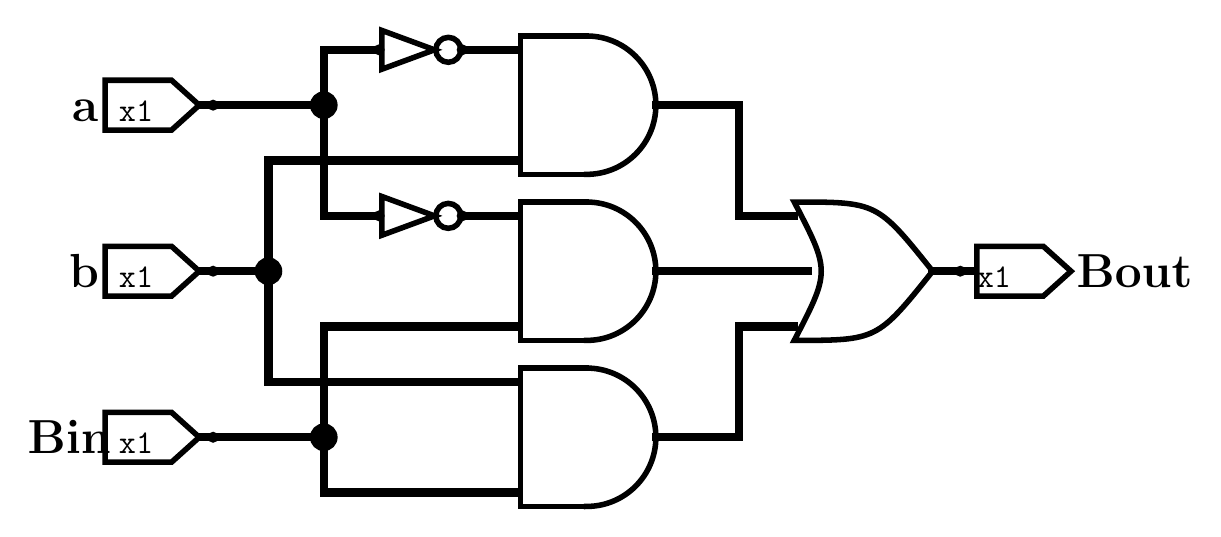
\begin{tikzpicture}[x=1pt,y=-1pt,line cap=rect]
\def\logisimfontA#1{\fontfamily{cmr}{#1}} % Replaced by logisim, original font was "SansSerif"
\def\logisimfontB#1{\fontfamily{cmtt}{#1}} % Replaced by logisim, original font was "Monospaced"
\definecolor{custcol_0_0_0}{RGB}{0, 0, 0}
\definecolor{custcol_ff_ff_ff}{RGB}{255, 255, 255}
\draw [line width=3.0pt, custcol_0_0_0 ]  (162.0,14.0) -- (182.0,14.0) ;
\draw [line width=3.0pt, custcol_0_0_0 ]  (162.0,74.0) -- (182.0,74.0) ;
\draw [line width=3.0pt, custcol_0_0_0 ]  (182.0,54.0) -- (92.0,54.0) -- (92.0,94.0) ;
\draw [line width=3.0pt, custcol_0_0_0 ]  (112.0,34.0) -- (112.0,74.0) -- (132.0,74.0) ;
\draw [line width=3.0pt, custcol_0_0_0 ]  (332.0,94.0) -- (342.0,94.0) ;
\draw [line width=3.0pt, custcol_0_0_0 ]  (112.0,154.0) -- (112.0,114.0) -- (182.0,114.0) ;
\fill [line width=3.0pt, custcol_0_0_0]  (112.0,154.0) ellipse (5.0 and 5.0 );
\fill [line width=3.0pt, custcol_0_0_0]  (112.0,34.0) ellipse (5.0 and 5.0 );
\fill [line width=3.0pt, custcol_0_0_0]  (92.0,94.0) ellipse (5.0 and 5.0 );
\draw [line width=2.0pt, custcol_0_0_0] (207.0,119.0) arc (90.0:-90.0:25.0 and 25.0 );
\draw [line width=2.0pt, custcol_0_0_0 ]  (207.0,69.0) -- (183.0,69.0) -- (183.0,119.0) -- (207.0,119.0) ;
\draw [line width=2.0pt, custcol_0_0_0] (207.0,179.0) arc (90.0:-90.0:25.0 and 25.0 );
\draw [line width=2.0pt, custcol_0_0_0 ]  (207.0,129.0) -- (183.0,129.0) -- (183.0,179.0) -- (207.0,179.0) ;
\draw [line width=2.0pt, custcol_0_0_0] (207.0,59.0) arc (90.0:-90.0:25.0 and 25.0 );
\draw [line width=2.0pt, custcol_0_0_0 ]  (207.0,9.0) -- (183.0,9.0) -- (183.0,59.0) -- (207.0,59.0) ;
\draw [line width=3.0pt, custcol_0_0_0 ]  (232.0,34.0) -- (262.0,34.0) -- (262.0,74.0) -- (282.0,74.0) -- (282.0,74.0) ;
\draw [line width=3.0pt, custcol_0_0_0 ]  (232.0,94.0) -- (282.0,94.0) -- (287.0,94.0) ;
\draw [line width=3.0pt, custcol_0_0_0 ]  (282.0,114.0) -- (282.0,114.0) -- (262.0,114.0) -- (262.0,154.0) -- (232.0,154.0) ;
\draw [line width=2.0pt, custcol_0_0_0 ]  (332.0,94.0) .. controls  (312.0,69.0)  ..  (282.0,69.0) .. controls  (295.0,94.0)  ..  (282.0,119.0) .. controls  (312.0,119.0)  ..  (332.0,94.0) -- cycle ;
\draw [line width=3.0pt, custcol_0_0_0 ]  (346.0,94.0) -- (343.0,94.0) ;
\draw [line width=2.0pt, custcol_0_0_0 ]  (372.0,85.0) -- (382.0,94.0) -- (372.0,103.0) -- (348.0,103.0) -- (348.0,85.0) -- cycle;
\logisimfontB{\fontsize{12pt}{12pt}\selectfont\node[inner sep=0, outer sep=0, custcol_0_0_0, anchor=base west] at  (348.0,100.0)  {x1};}
\logisimfontA{\fontsize{16pt}{16pt}\fontseries{bx}\selectfont\node[inner sep=0, outer sep=0, custcol_0_0_0, anchor=base west] at  (384.0,100.0)  {Bout};}
\fill [line width=2.0pt, custcol_0_0_0]  (342.0,94.0) ellipse (2.0 and 2.0 );
\draw [line width=2.0pt, custcol_0_0_0 ]  (152.0,14.0) -- (133.0,7.0) -- (133.0,21.0) -- cycle;
\draw [line width=2.0pt, custcol_0_0_0]  (157.0,14.0) ellipse (4.5 and 4.5 );
\fill [line width=2.0pt, custcol_0_0_0]  (162.0,14.0) ellipse (2.0 and 2.0 );
\fill [line width=2.0pt, custcol_0_0_0]  (132.0,14.0) ellipse (2.0 and 2.0 );
\draw [line width=2.0pt, custcol_0_0_0 ]  (152.0,74.0) -- (133.0,67.0) -- (133.0,81.0) -- cycle;
\draw [line width=2.0pt, custcol_0_0_0]  (157.0,74.0) ellipse (4.5 and 4.5 );
\fill [line width=2.0pt, custcol_0_0_0]  (162.0,74.0) ellipse (2.0 and 2.0 );
\fill [line width=2.0pt, custcol_0_0_0]  (132.0,74.0) ellipse (2.0 and 2.0 );
\draw [line width=3.0pt, custcol_0_0_0 ]  (67.0,154.0) -- (72.0,154.0) -- (112.0,154.0) -- (112.0,174.0) -- (182.0,174.0) ;
\draw [line width=2.0pt, custcol_0_0_0 ]  (57.0,163.0) -- (67.0,154.0) -- (57.0,145.0) -- (33.0,145.0) -- (33.0,163.0) -- cycle;
\logisimfontB{\fontsize{12pt}{12pt}\selectfont\node[inner sep=0, outer sep=0, custcol_0_0_0, anchor=base west] at  (38.0,160.0)  {x1};}
\logisimfontA{\fontsize{16pt}{16pt}\fontseries{bx}\selectfont\node[inner sep=0, outer sep=0, custcol_0_0_0, anchor=base west] at  (5.0,160.0)  {Bin};}
\fill [line width=2.0pt, custcol_0_0_0]  (72.0,154.0) ellipse (2.0 and 2.0 );
\draw [line width=3.0pt, custcol_0_0_0 ]  (67.0,94.0) -- (72.0,94.0) -- (92.0,94.0) -- (92.0,134.0) -- (182.0,134.0) ;
\draw [line width=2.0pt, custcol_0_0_0 ]  (57.0,103.0) -- (67.0,94.0) -- (57.0,85.0) -- (33.0,85.0) -- (33.0,103.0) -- cycle;
\logisimfontB{\fontsize{12pt}{12pt}\selectfont\node[inner sep=0, outer sep=0, custcol_0_0_0, anchor=base west] at  (38.0,100.0)  {x1};}
\logisimfontA{\fontsize{16pt}{16pt}\fontseries{bx}\selectfont\node[inner sep=0, outer sep=0, custcol_0_0_0, anchor=base west] at  (20.0,100.0)  {b};}
\fill [line width=2.0pt, custcol_0_0_0]  (72.0,94.0) ellipse (2.0 and 2.0 );
\draw [line width=3.0pt, custcol_0_0_0 ]  (67.0,34.0) -- (72.0,34.0) -- (112.0,34.0) -- (112.0,14.0) -- (132.0,14.0) ;
\draw [line width=2.0pt, custcol_0_0_0 ]  (57.0,43.0) -- (67.0,34.0) -- (57.0,25.0) -- (33.0,25.0) -- (33.0,43.0) -- cycle;
\logisimfontB{\fontsize{12pt}{12pt}\selectfont\node[inner sep=0, outer sep=0, custcol_0_0_0, anchor=base west] at  (38.0,40.0)  {x1};}
\logisimfontA{\fontsize{16pt}{16pt}\fontseries{bx}\selectfont\node[inner sep=0, outer sep=0, custcol_0_0_0, anchor=base west] at  (21.0,40.0)  {a};}
\fill [line width=2.0pt, custcol_0_0_0]  (72.0,34.0) ellipse (2.0 and 2.0 );
\end{tikzpicture}
}

		\label{fig:subtratorcompletoparte02}
	\end{figure}
\end{frame}

\begin{frame}
	\frametitle{Subtrator completo}
	\framesubtitle{\textbf{Prática dirigida}}
	\par Portanto o circuito \textbf{subtrator completo} ou \textbf{Full subtractor} fica assim:
	\begin{figure}
		\centering
		% Important: If latex complains about unicode characters,
% please use "\usepackage[utf8x]{inputenc}" in your preamble
% You can change the size of the picture by putting it into the construct:
% 1) \resizebox{10cm}{!}{"below picture"} to scale horizontally to 10 cm
% 2) \resizebox{!}{15cm}{"below picture"} to scale vertically to 15 cm
% 3) \resizebox{10cm}{15cm}{"below picture"} a combination of above two
% It is not recomended to use the scale option of the tikzpicture environment.
 \resizebox{7cm}{!}{
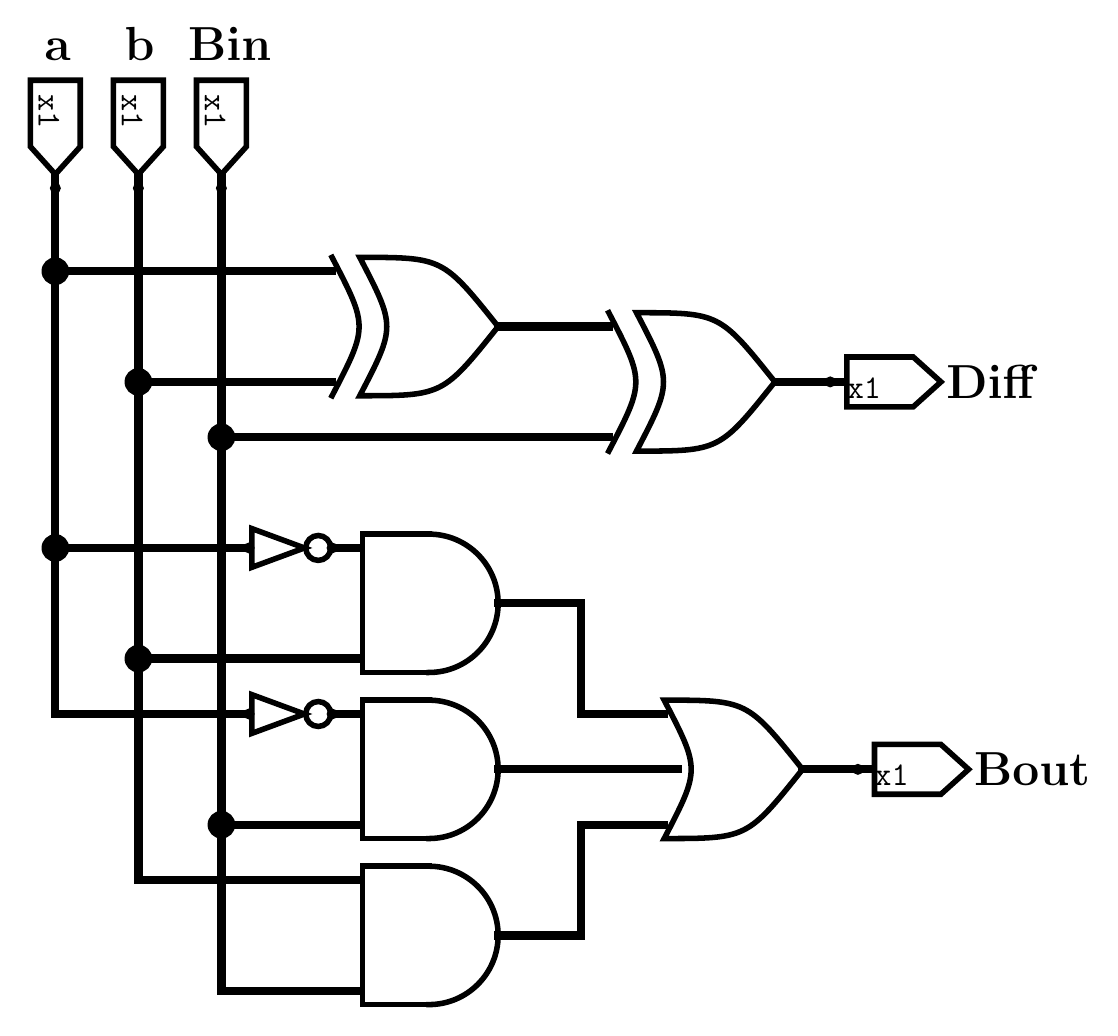
\begin{tikzpicture}[x=1pt,y=-1pt,line cap=rect]
\def\logisimfontA#1{\fontfamily{cmr}{#1}} % Replaced by logisim, original font was "SansSerif"
\def\logisimfontB#1{\fontfamily{cmtt}{#1}} % Replaced by logisim, original font was "Monospaced"
\definecolor{custcol_0_0_0}{RGB}{0, 0, 0}
\definecolor{custcol_ff_ff_ff}{RGB}{255, 255, 255}
\draw [line width=3.0pt, custcol_0_0_0 ]  (275.0,134.0) -- (295.0,134.0) ;
\draw [line width=3.0pt, custcol_0_0_0 ]  (285.0,274.0) -- (305.0,274.0) ;
\draw [line width=3.0pt, custcol_0_0_0 ]  (115.0,254.0) -- (125.0,254.0) ;
\draw [line width=3.0pt, custcol_0_0_0 ]  (115.0,194.0) -- (125.0,194.0) ;
\draw [line width=3.0pt, custcol_0_0_0 ]  (45.0,234.0) -- (125.0,234.0) ;
\draw [line width=3.0pt, custcol_0_0_0 ]  (75.0,294.0) -- (75.0,354.0) -- (125.0,354.0) ;
\draw [line width=3.0pt, custcol_0_0_0 ]  (15.0,194.0) -- (85.0,194.0) ;
\draw [line width=3.0pt, custcol_0_0_0 ]  (15.0,94.0) -- (15.0,194.0) -- (15.0,254.0) -- (85.0,254.0) ;
\fill [line width=3.0pt, custcol_0_0_0]  (45.0,134.0) ellipse (5.0 and 5.0 );
\fill [line width=3.0pt, custcol_0_0_0]  (75.0,294.0) ellipse (5.0 and 5.0 );
\fill [line width=3.0pt, custcol_0_0_0]  (15.0,194.0) ellipse (5.0 and 5.0 );
\fill [line width=3.0pt, custcol_0_0_0]  (45.0,234.0) ellipse (5.0 and 5.0 );
\fill [line width=3.0pt, custcol_0_0_0]  (15.0,94.0) ellipse (5.0 and 5.0 );
\fill [line width=3.0pt, custcol_0_0_0]  (75.0,154.0) ellipse (5.0 and 5.0 );
\draw [line width=2.0pt, custcol_0_0_0 ]  (6.0,49.0) -- (15.0,59.0) -- (24.0,49.0) -- (24.0,25.0) -- (6.0,25.0) -- cycle;
\logisimfontB{\fontsize{12pt}{12pt}\selectfont\node[inner sep=0, outer sep=0, custcol_0_0_0, anchor=base west, rotate=-90.0] at  (9.0,30.0)  {x1};}
\logisimfontA{\fontsize{16pt}{16pt}\fontseries{bx}\selectfont\node[inner sep=0, outer sep=0, custcol_0_0_0, anchor=base west] at  (11.0,18.0)  {a};}
\fill [line width=2.0pt, custcol_0_0_0]  (15.0,64.0) ellipse (2.0 and 2.0 );
\draw [line width=3.0pt, custcol_0_0_0 ]  (45.0,59.0) -- (45.0,64.0) -- (45.0,134.0) -- (45.0,234.0) -- (45.0,314.0) -- (125.0,314.0) ;
\draw [line width=2.0pt, custcol_0_0_0 ]  (36.0,49.0) -- (45.0,59.0) -- (54.0,49.0) -- (54.0,25.0) -- (36.0,25.0) -- cycle;
\logisimfontB{\fontsize{12pt}{12pt}\selectfont\node[inner sep=0, outer sep=0, custcol_0_0_0, anchor=base west, rotate=-90.0] at  (39.0,30.0)  {x1};}
\logisimfontA{\fontsize{16pt}{16pt}\fontseries{bx}\selectfont\node[inner sep=0, outer sep=0, custcol_0_0_0, anchor=base west] at  (40.0,18.0)  {b};}
\fill [line width=2.0pt, custcol_0_0_0]  (45.0,64.0) ellipse (2.0 and 2.0 );
\draw [line width=3.0pt, custcol_0_0_0 ]  (75.0,59.0) -- (75.0,64.0) -- (75.0,154.0) -- (75.0,294.0) -- (125.0,294.0) ;
\draw [line width=2.0pt, custcol_0_0_0 ]  (66.0,49.0) -- (75.0,59.0) -- (84.0,49.0) -- (84.0,25.0) -- (66.0,25.0) -- cycle;
\logisimfontB{\fontsize{12pt}{12pt}\selectfont\node[inner sep=0, outer sep=0, custcol_0_0_0, anchor=base west, rotate=-90.0] at  (69.0,30.0)  {x1};}
\logisimfontA{\fontsize{16pt}{16pt}\fontseries{bx}\selectfont\node[inner sep=0, outer sep=0, custcol_0_0_0, anchor=base west] at  (63.0,18.0)  {Bin};}
\fill [line width=2.0pt, custcol_0_0_0]  (75.0,64.0) ellipse (2.0 and 2.0 );
\draw [line width=3.0pt, custcol_0_0_0 ]  (299.0,134.0) -- (296.0,134.0) ;
\draw [line width=2.0pt, custcol_0_0_0 ]  (325.0,125.0) -- (335.0,134.0) -- (325.0,143.0) -- (301.0,143.0) -- (301.0,125.0) -- cycle;
\logisimfontB{\fontsize{12pt}{12pt}\selectfont\node[inner sep=0, outer sep=0, custcol_0_0_0, anchor=base west] at  (301.0,140.0)  {x1};}
\logisimfontA{\fontsize{16pt}{16pt}\fontseries{bx}\selectfont\node[inner sep=0, outer sep=0, custcol_0_0_0, anchor=base west] at  (337.0,140.0)  {Diff};}
\fill [line width=2.0pt, custcol_0_0_0]  (295.0,134.0) ellipse (2.0 and 2.0 );
\draw [line width=3.0pt, custcol_0_0_0 ]  (15.0,59.0) -- (15.0,64.0) -- (15.0,94.0) -- (115.0,94.0) -- (115.0,94.0) ;
\draw [line width=3.0pt, custcol_0_0_0 ]  (45.0,134.0) -- (115.0,134.0) -- (115.0,134.0) ;
\draw [line width=2.0pt, custcol_0_0_0 ]  (175.0,114.0) .. controls  (155.0,89.0)  ..  (125.0,89.0) .. controls  (138.0,114.0)  ..  (125.0,139.0) .. controls  (155.0,139.0)  ..  (175.0,114.0) -- cycle ;
\draw [line width=2.0pt, custcol_0_0_0 ]  (115.0,89.0) .. controls  (128.0,114.0)  ..  (115.0,139.0) ;
\draw [line width=3.0pt, custcol_0_0_0 ]  (175.0,114.0) -- (215.0,114.0) -- (215.0,114.0) ;
\draw [line width=3.0pt, custcol_0_0_0 ]  (75.0,154.0) -- (215.0,154.0) -- (215.0,154.0) ;
\draw [line width=2.0pt, custcol_0_0_0 ]  (275.0,134.0) .. controls  (255.0,109.0)  ..  (225.0,109.0) .. controls  (238.0,134.0)  ..  (225.0,159.0) .. controls  (255.0,159.0)  ..  (275.0,134.0) -- cycle ;
\draw [line width=2.0pt, custcol_0_0_0 ]  (215.0,109.0) .. controls  (228.0,134.0)  ..  (215.0,159.0) ;
\draw [line width=2.0pt, custcol_0_0_0 ]  (105.0,194.0) -- (86.0,187.0) -- (86.0,201.0) -- cycle;
\draw [line width=2.0pt, custcol_0_0_0]  (110.0,194.0) ellipse (4.5 and 4.5 );
\fill [line width=2.0pt, custcol_0_0_0]  (115.0,194.0) ellipse (2.0 and 2.0 );
\fill [line width=2.0pt, custcol_0_0_0]  (85.0,194.0) ellipse (2.0 and 2.0 );
\draw [line width=3.0pt, custcol_0_0_0 ]  (309.0,274.0) -- (306.0,274.0) ;
\draw [line width=2.0pt, custcol_0_0_0 ]  (335.0,265.0) -- (345.0,274.0) -- (335.0,283.0) -- (311.0,283.0) -- (311.0,265.0) -- cycle;
\logisimfontB{\fontsize{12pt}{12pt}\selectfont\node[inner sep=0, outer sep=0, custcol_0_0_0, anchor=base west] at  (311.0,280.0)  {x1};}
\logisimfontA{\fontsize{16pt}{16pt}\fontseries{bx}\selectfont\node[inner sep=0, outer sep=0, custcol_0_0_0, anchor=base west] at  (347.0,280.0)  {Bout};}
\fill [line width=2.0pt, custcol_0_0_0]  (305.0,274.0) ellipse (2.0 and 2.0 );
\draw [line width=2.0pt, custcol_0_0_0] (150.0,239.0) arc (90.0:-90.0:25.0 and 25.0 );
\draw [line width=2.0pt, custcol_0_0_0 ]  (150.0,189.0) -- (126.0,189.0) -- (126.0,239.0) -- (150.0,239.0) ;
\draw [line width=2.0pt, custcol_0_0_0] (150.0,359.0) arc (90.0:-90.0:25.0 and 25.0 );
\draw [line width=2.0pt, custcol_0_0_0 ]  (150.0,309.0) -- (126.0,309.0) -- (126.0,359.0) -- (150.0,359.0) ;
\draw [line width=2.0pt, custcol_0_0_0] (150.0,299.0) arc (90.0:-90.0:25.0 and 25.0 );
\draw [line width=2.0pt, custcol_0_0_0 ]  (150.0,249.0) -- (126.0,249.0) -- (126.0,299.0) -- (150.0,299.0) ;
\draw [line width=3.0pt, custcol_0_0_0 ]  (175.0,214.0) -- (205.0,214.0) -- (205.0,254.0) -- (235.0,254.0) -- (235.0,254.0) ;
\draw [line width=3.0pt, custcol_0_0_0 ]  (175.0,274.0) -- (235.0,274.0) -- (240.0,274.0) ;
\draw [line width=3.0pt, custcol_0_0_0 ]  (235.0,294.0) -- (235.0,294.0) -- (205.0,294.0) -- (205.0,334.0) -- (175.0,334.0) ;
\draw [line width=2.0pt, custcol_0_0_0 ]  (285.0,274.0) .. controls  (265.0,249.0)  ..  (235.0,249.0) .. controls  (248.0,274.0)  ..  (235.0,299.0) .. controls  (265.0,299.0)  ..  (285.0,274.0) -- cycle ;
\draw [line width=2.0pt, custcol_0_0_0 ]  (105.0,254.0) -- (86.0,247.0) -- (86.0,261.0) -- cycle;
\draw [line width=2.0pt, custcol_0_0_0]  (110.0,254.0) ellipse (4.5 and 4.5 );
\fill [line width=2.0pt, custcol_0_0_0]  (115.0,254.0) ellipse (2.0 and 2.0 );
\fill [line width=2.0pt, custcol_0_0_0]  (85.0,254.0) ellipse (2.0 and 2.0 );
\end{tikzpicture}
}

		\label{fig:subtratorcompleto}
	\end{figure}
\end{frame}

\section{Mas... mas... \textit{Oh... wait a fucking moment!}}

\begin{frame}
	\frametitle{KKKKKKKK}
	\begin{columns}
		\column{.5\linewidth}
			\begin{figure}
			\centering
			% Important: If latex complains about unicode characters,
% please use "\usepackage[utf8x]{inputenc}" in your preamble
% You can change the size of the picture by putting it into the construct:
% 1) \resizebox{10cm}{!}{"below picture"} to scale horizontally to 10 cm
% 2) \resizebox{!}{15cm}{"below picture"} to scale vertically to 15 cm
% 3) \resizebox{10cm}{15cm}{"below picture"} a combination of above two
% It is not recomended to use the scale option of the tikzpicture environment.
 \resizebox{7cm}{!}{
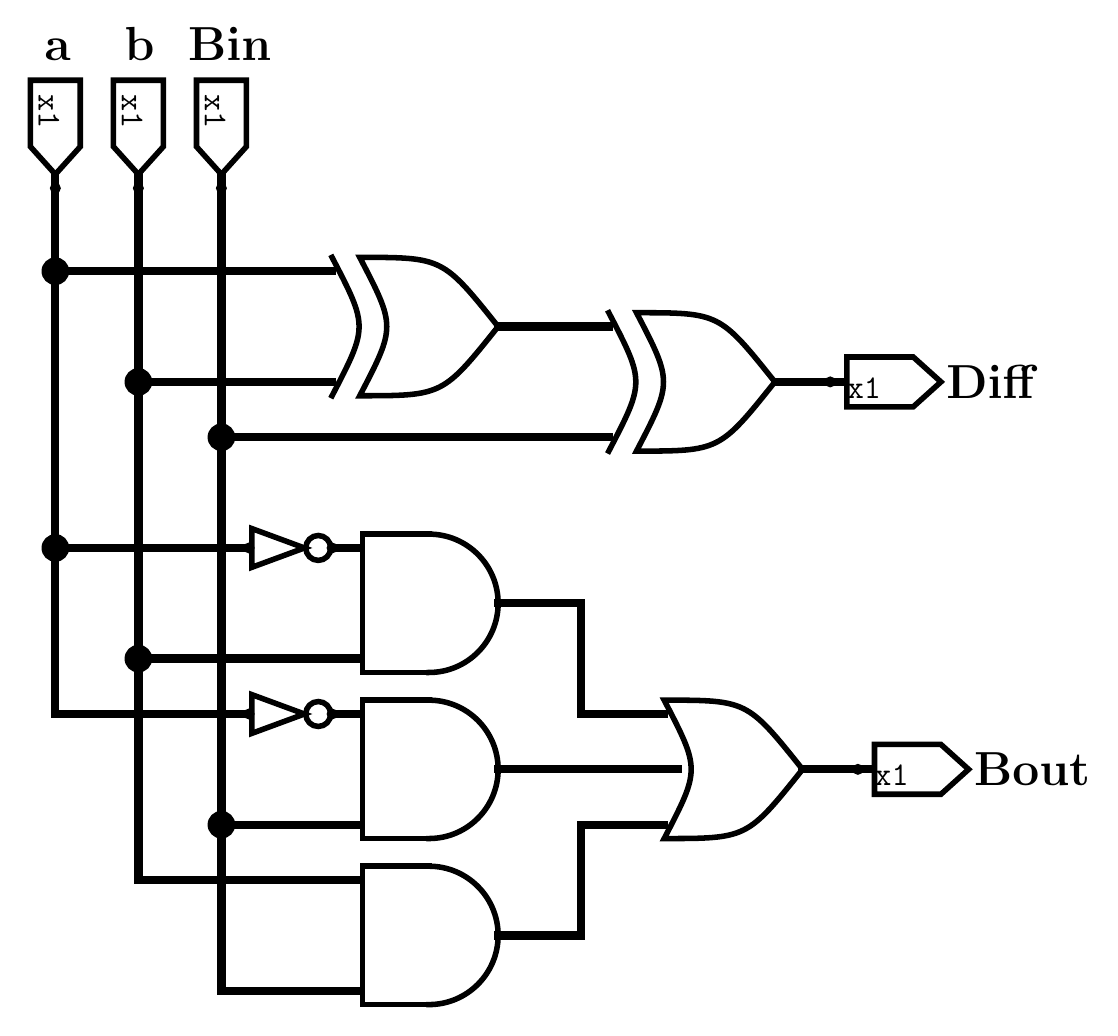
\begin{tikzpicture}[x=1pt,y=-1pt,line cap=rect]
\def\logisimfontA#1{\fontfamily{cmr}{#1}} % Replaced by logisim, original font was "SansSerif"
\def\logisimfontB#1{\fontfamily{cmtt}{#1}} % Replaced by logisim, original font was "Monospaced"
\definecolor{custcol_0_0_0}{RGB}{0, 0, 0}
\definecolor{custcol_ff_ff_ff}{RGB}{255, 255, 255}
\draw [line width=3.0pt, custcol_0_0_0 ]  (275.0,134.0) -- (295.0,134.0) ;
\draw [line width=3.0pt, custcol_0_0_0 ]  (285.0,274.0) -- (305.0,274.0) ;
\draw [line width=3.0pt, custcol_0_0_0 ]  (115.0,254.0) -- (125.0,254.0) ;
\draw [line width=3.0pt, custcol_0_0_0 ]  (115.0,194.0) -- (125.0,194.0) ;
\draw [line width=3.0pt, custcol_0_0_0 ]  (45.0,234.0) -- (125.0,234.0) ;
\draw [line width=3.0pt, custcol_0_0_0 ]  (75.0,294.0) -- (75.0,354.0) -- (125.0,354.0) ;
\draw [line width=3.0pt, custcol_0_0_0 ]  (15.0,194.0) -- (85.0,194.0) ;
\draw [line width=3.0pt, custcol_0_0_0 ]  (15.0,94.0) -- (15.0,194.0) -- (15.0,254.0) -- (85.0,254.0) ;
\fill [line width=3.0pt, custcol_0_0_0]  (45.0,134.0) ellipse (5.0 and 5.0 );
\fill [line width=3.0pt, custcol_0_0_0]  (75.0,294.0) ellipse (5.0 and 5.0 );
\fill [line width=3.0pt, custcol_0_0_0]  (15.0,194.0) ellipse (5.0 and 5.0 );
\fill [line width=3.0pt, custcol_0_0_0]  (45.0,234.0) ellipse (5.0 and 5.0 );
\fill [line width=3.0pt, custcol_0_0_0]  (15.0,94.0) ellipse (5.0 and 5.0 );
\fill [line width=3.0pt, custcol_0_0_0]  (75.0,154.0) ellipse (5.0 and 5.0 );
\draw [line width=2.0pt, custcol_0_0_0 ]  (6.0,49.0) -- (15.0,59.0) -- (24.0,49.0) -- (24.0,25.0) -- (6.0,25.0) -- cycle;
\logisimfontB{\fontsize{12pt}{12pt}\selectfont\node[inner sep=0, outer sep=0, custcol_0_0_0, anchor=base west, rotate=-90.0] at  (9.0,30.0)  {x1};}
\logisimfontA{\fontsize{16pt}{16pt}\fontseries{bx}\selectfont\node[inner sep=0, outer sep=0, custcol_0_0_0, anchor=base west] at  (11.0,18.0)  {a};}
\fill [line width=2.0pt, custcol_0_0_0]  (15.0,64.0) ellipse (2.0 and 2.0 );
\draw [line width=3.0pt, custcol_0_0_0 ]  (45.0,59.0) -- (45.0,64.0) -- (45.0,134.0) -- (45.0,234.0) -- (45.0,314.0) -- (125.0,314.0) ;
\draw [line width=2.0pt, custcol_0_0_0 ]  (36.0,49.0) -- (45.0,59.0) -- (54.0,49.0) -- (54.0,25.0) -- (36.0,25.0) -- cycle;
\logisimfontB{\fontsize{12pt}{12pt}\selectfont\node[inner sep=0, outer sep=0, custcol_0_0_0, anchor=base west, rotate=-90.0] at  (39.0,30.0)  {x1};}
\logisimfontA{\fontsize{16pt}{16pt}\fontseries{bx}\selectfont\node[inner sep=0, outer sep=0, custcol_0_0_0, anchor=base west] at  (40.0,18.0)  {b};}
\fill [line width=2.0pt, custcol_0_0_0]  (45.0,64.0) ellipse (2.0 and 2.0 );
\draw [line width=3.0pt, custcol_0_0_0 ]  (75.0,59.0) -- (75.0,64.0) -- (75.0,154.0) -- (75.0,294.0) -- (125.0,294.0) ;
\draw [line width=2.0pt, custcol_0_0_0 ]  (66.0,49.0) -- (75.0,59.0) -- (84.0,49.0) -- (84.0,25.0) -- (66.0,25.0) -- cycle;
\logisimfontB{\fontsize{12pt}{12pt}\selectfont\node[inner sep=0, outer sep=0, custcol_0_0_0, anchor=base west, rotate=-90.0] at  (69.0,30.0)  {x1};}
\logisimfontA{\fontsize{16pt}{16pt}\fontseries{bx}\selectfont\node[inner sep=0, outer sep=0, custcol_0_0_0, anchor=base west] at  (63.0,18.0)  {Bin};}
\fill [line width=2.0pt, custcol_0_0_0]  (75.0,64.0) ellipse (2.0 and 2.0 );
\draw [line width=3.0pt, custcol_0_0_0 ]  (299.0,134.0) -- (296.0,134.0) ;
\draw [line width=2.0pt, custcol_0_0_0 ]  (325.0,125.0) -- (335.0,134.0) -- (325.0,143.0) -- (301.0,143.0) -- (301.0,125.0) -- cycle;
\logisimfontB{\fontsize{12pt}{12pt}\selectfont\node[inner sep=0, outer sep=0, custcol_0_0_0, anchor=base west] at  (301.0,140.0)  {x1};}
\logisimfontA{\fontsize{16pt}{16pt}\fontseries{bx}\selectfont\node[inner sep=0, outer sep=0, custcol_0_0_0, anchor=base west] at  (337.0,140.0)  {Diff};}
\fill [line width=2.0pt, custcol_0_0_0]  (295.0,134.0) ellipse (2.0 and 2.0 );
\draw [line width=3.0pt, custcol_0_0_0 ]  (15.0,59.0) -- (15.0,64.0) -- (15.0,94.0) -- (115.0,94.0) -- (115.0,94.0) ;
\draw [line width=3.0pt, custcol_0_0_0 ]  (45.0,134.0) -- (115.0,134.0) -- (115.0,134.0) ;
\draw [line width=2.0pt, custcol_0_0_0 ]  (175.0,114.0) .. controls  (155.0,89.0)  ..  (125.0,89.0) .. controls  (138.0,114.0)  ..  (125.0,139.0) .. controls  (155.0,139.0)  ..  (175.0,114.0) -- cycle ;
\draw [line width=2.0pt, custcol_0_0_0 ]  (115.0,89.0) .. controls  (128.0,114.0)  ..  (115.0,139.0) ;
\draw [line width=3.0pt, custcol_0_0_0 ]  (175.0,114.0) -- (215.0,114.0) -- (215.0,114.0) ;
\draw [line width=3.0pt, custcol_0_0_0 ]  (75.0,154.0) -- (215.0,154.0) -- (215.0,154.0) ;
\draw [line width=2.0pt, custcol_0_0_0 ]  (275.0,134.0) .. controls  (255.0,109.0)  ..  (225.0,109.0) .. controls  (238.0,134.0)  ..  (225.0,159.0) .. controls  (255.0,159.0)  ..  (275.0,134.0) -- cycle ;
\draw [line width=2.0pt, custcol_0_0_0 ]  (215.0,109.0) .. controls  (228.0,134.0)  ..  (215.0,159.0) ;
\draw [line width=2.0pt, custcol_0_0_0 ]  (105.0,194.0) -- (86.0,187.0) -- (86.0,201.0) -- cycle;
\draw [line width=2.0pt, custcol_0_0_0]  (110.0,194.0) ellipse (4.5 and 4.5 );
\fill [line width=2.0pt, custcol_0_0_0]  (115.0,194.0) ellipse (2.0 and 2.0 );
\fill [line width=2.0pt, custcol_0_0_0]  (85.0,194.0) ellipse (2.0 and 2.0 );
\draw [line width=3.0pt, custcol_0_0_0 ]  (309.0,274.0) -- (306.0,274.0) ;
\draw [line width=2.0pt, custcol_0_0_0 ]  (335.0,265.0) -- (345.0,274.0) -- (335.0,283.0) -- (311.0,283.0) -- (311.0,265.0) -- cycle;
\logisimfontB{\fontsize{12pt}{12pt}\selectfont\node[inner sep=0, outer sep=0, custcol_0_0_0, anchor=base west] at  (311.0,280.0)  {x1};}
\logisimfontA{\fontsize{16pt}{16pt}\fontseries{bx}\selectfont\node[inner sep=0, outer sep=0, custcol_0_0_0, anchor=base west] at  (347.0,280.0)  {Bout};}
\fill [line width=2.0pt, custcol_0_0_0]  (305.0,274.0) ellipse (2.0 and 2.0 );
\draw [line width=2.0pt, custcol_0_0_0] (150.0,239.0) arc (90.0:-90.0:25.0 and 25.0 );
\draw [line width=2.0pt, custcol_0_0_0 ]  (150.0,189.0) -- (126.0,189.0) -- (126.0,239.0) -- (150.0,239.0) ;
\draw [line width=2.0pt, custcol_0_0_0] (150.0,359.0) arc (90.0:-90.0:25.0 and 25.0 );
\draw [line width=2.0pt, custcol_0_0_0 ]  (150.0,309.0) -- (126.0,309.0) -- (126.0,359.0) -- (150.0,359.0) ;
\draw [line width=2.0pt, custcol_0_0_0] (150.0,299.0) arc (90.0:-90.0:25.0 and 25.0 );
\draw [line width=2.0pt, custcol_0_0_0 ]  (150.0,249.0) -- (126.0,249.0) -- (126.0,299.0) -- (150.0,299.0) ;
\draw [line width=3.0pt, custcol_0_0_0 ]  (175.0,214.0) -- (205.0,214.0) -- (205.0,254.0) -- (235.0,254.0) -- (235.0,254.0) ;
\draw [line width=3.0pt, custcol_0_0_0 ]  (175.0,274.0) -- (235.0,274.0) -- (240.0,274.0) ;
\draw [line width=3.0pt, custcol_0_0_0 ]  (235.0,294.0) -- (235.0,294.0) -- (205.0,294.0) -- (205.0,334.0) -- (175.0,334.0) ;
\draw [line width=2.0pt, custcol_0_0_0 ]  (285.0,274.0) .. controls  (265.0,249.0)  ..  (235.0,249.0) .. controls  (248.0,274.0)  ..  (235.0,299.0) .. controls  (265.0,299.0)  ..  (285.0,274.0) -- cycle ;
\draw [line width=2.0pt, custcol_0_0_0 ]  (105.0,254.0) -- (86.0,247.0) -- (86.0,261.0) -- cycle;
\draw [line width=2.0pt, custcol_0_0_0]  (110.0,254.0) ellipse (4.5 and 4.5 );
\fill [line width=2.0pt, custcol_0_0_0]  (115.0,254.0) ellipse (2.0 and 2.0 );
\fill [line width=2.0pt, custcol_0_0_0]  (85.0,254.0) ellipse (2.0 and 2.0 );
\end{tikzpicture}
}

			\label{fig:subtratorcompleto2}
		\end{figure}
		\column{.5\linewidth}
			\begin{figure}
			\centering
			% Important: If latex complains about unicode characters,
% please use "\usepackage[utf8x]{inputenc}" in your preamble
% You can change the size of the picture by putting it into the construct:
% 1) \resizebox{10cm}{!}{"below picture"} to scale horizontally to 10 cm
% 2) \resizebox{!}{15cm}{"below picture"} to scale vertically to 15 cm
% 3) \resizebox{10cm}{15cm}{"below picture"} a combination of above two
% It is not recomended to use the scale option of the tikzpicture environment.
\resizebox{7cm}{!}{
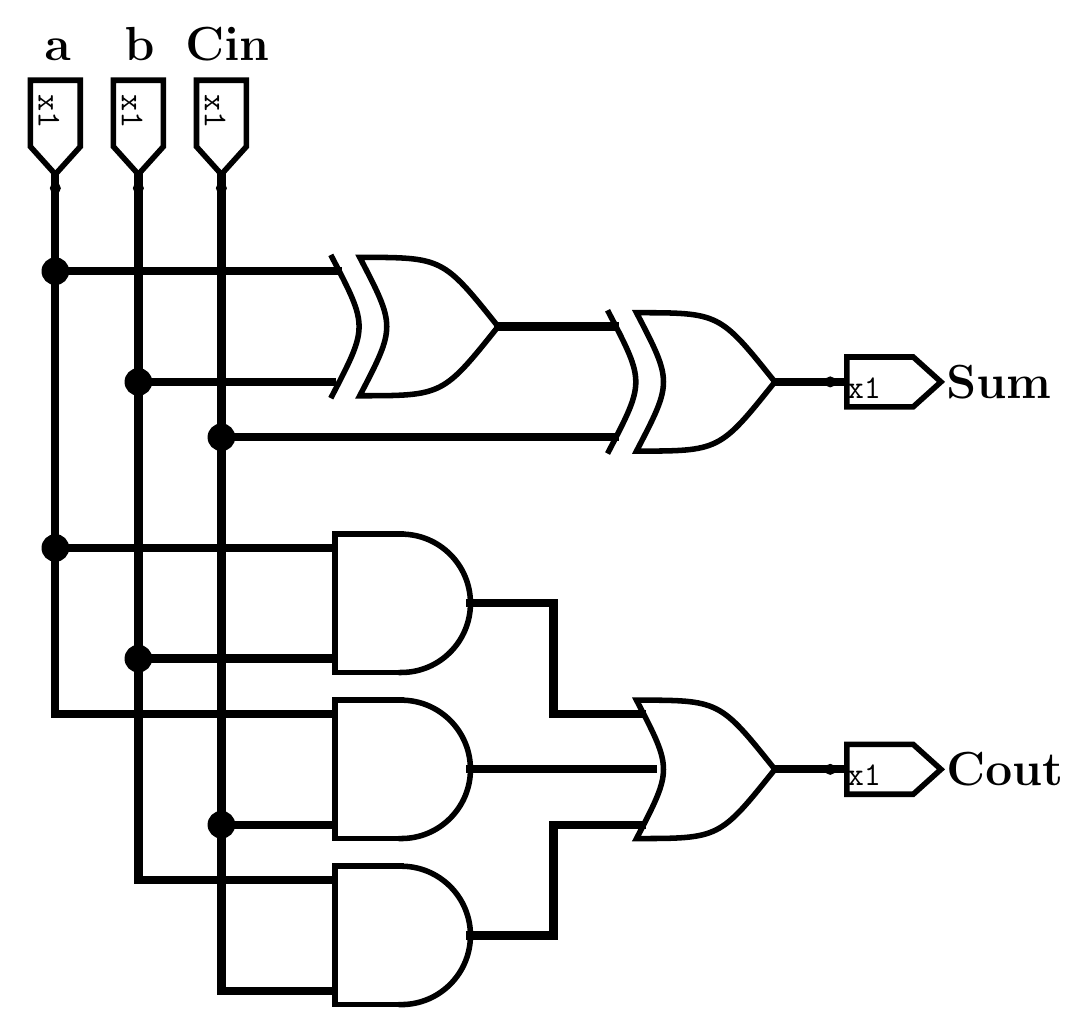
\begin{tikzpicture}[x=1pt,y=-1pt,line cap=rect]
\def\logisimfontA#1{\fontfamily{cmr}{#1}} % Replaced by logisim, original font was "SansSerif"
\def\logisimfontB#1{\fontfamily{cmtt}{#1}} % Replaced by logisim, original font was "Monospaced"
\definecolor{custcol_0_0_0}{RGB}{0, 0, 0}
\definecolor{custcol_ff_ff_ff}{RGB}{255, 255, 255}
\draw [line width=3.0pt, custcol_0_0_0 ]  (15.0,94.0) -- (15.0,194.0) -- (115.0,194.0) ;
\draw [line width=3.0pt, custcol_0_0_0 ]  (275.0,134.0) -- (295.0,134.0) ;
\draw [line width=3.0pt, custcol_0_0_0 ]  (275.0,274.0) -- (295.0,274.0) ;
\draw [line width=3.0pt, custcol_0_0_0 ]  (15.0,194.0) -- (15.0,254.0) -- (115.0,254.0) ;
\draw [line width=3.0pt, custcol_0_0_0 ]  (75.0,294.0) -- (75.0,354.0) -- (115.0,354.0) ;
\draw [line width=3.0pt, custcol_0_0_0 ]  (45.0,234.0) -- (115.0,234.0) ;
\fill [line width=3.0pt, custcol_0_0_0]  (45.0,134.0) ellipse (5.0 and 5.0 );
\fill [line width=3.0pt, custcol_0_0_0]  (15.0,194.0) ellipse (5.0 and 5.0 );
\fill [line width=3.0pt, custcol_0_0_0]  (75.0,154.0) ellipse (5.0 and 5.0 );
\fill [line width=3.0pt, custcol_0_0_0]  (15.0,94.0) ellipse (5.0 and 5.0 );
\fill [line width=3.0pt, custcol_0_0_0]  (75.0,294.0) ellipse (5.0 and 5.0 );
\fill [line width=3.0pt, custcol_0_0_0]  (45.0,234.0) ellipse (5.0 and 5.0 );
\draw [line width=3.0pt, custcol_0_0_0 ]  (75.0,59.0) -- (75.0,64.0) -- (75.0,154.0) -- (75.0,294.0) -- (115.0,294.0) ;
\draw [line width=2.0pt, custcol_0_0_0 ]  (66.0,49.0) -- (75.0,59.0) -- (84.0,49.0) -- (84.0,25.0) -- (66.0,25.0) -- cycle;
\logisimfontB{\fontsize{12pt}{12pt}\selectfont\node[inner sep=0, outer sep=0, custcol_0_0_0, anchor=base west, rotate=-90.0] at  (69.0,30.0)  {x1};}
\logisimfontA{\fontsize{16pt}{16pt}\fontseries{bx}\selectfont\node[inner sep=0, outer sep=0, custcol_0_0_0, anchor=base west] at  (62.0,18.0)  {Cin};}
\fill [line width=2.0pt, custcol_0_0_0]  (75.0,64.0) ellipse (2.0 and 2.0 );
\draw [line width=2.0pt, custcol_0_0_0 ]  (6.0,49.0) -- (15.0,59.0) -- (24.0,49.0) -- (24.0,25.0) -- (6.0,25.0) -- cycle;
\logisimfontB{\fontsize{12pt}{12pt}\selectfont\node[inner sep=0, outer sep=0, custcol_0_0_0, anchor=base west, rotate=-90.0] at  (9.0,30.0)  {x1};}
\logisimfontA{\fontsize{16pt}{16pt}\fontseries{bx}\selectfont\node[inner sep=0, outer sep=0, custcol_0_0_0, anchor=base west] at  (11.0,18.0)  {a};}
\fill [line width=2.0pt, custcol_0_0_0]  (15.0,64.0) ellipse (2.0 and 2.0 );
\draw [line width=2.0pt, custcol_0_0_0] (140.0,359.0) arc (90.0:-90.0:25.0 and 25.0 );
\draw [line width=2.0pt, custcol_0_0_0 ]  (140.0,309.0) -- (116.0,309.0) -- (116.0,359.0) -- (140.0,359.0) ;
\draw [line width=3.0pt, custcol_0_0_0 ]  (165.0,214.0) -- (195.0,214.0) -- (195.0,254.0) -- (225.0,254.0) -- (227.0,254.0) ;
\draw [line width=3.0pt, custcol_0_0_0 ]  (165.0,274.0) -- (225.0,274.0) -- (231.0,274.0) ;
\draw [line width=3.0pt, custcol_0_0_0 ]  (165.0,334.0) -- (195.0,334.0) -- (195.0,294.0) -- (225.0,294.0) -- (227.0,294.0) ;
\draw [line width=2.0pt, custcol_0_0_0 ]  (275.0,274.0) .. controls  (255.0,249.0)  ..  (225.0,249.0) .. controls  (238.0,274.0)  ..  (225.0,299.0) .. controls  (255.0,299.0)  ..  (275.0,274.0) -- cycle ;
\draw [line width=3.0pt, custcol_0_0_0 ]  (175.0,114.0) -- (215.0,114.0) -- (217.0,114.0) ;
\draw [line width=3.0pt, custcol_0_0_0 ]  (75.0,154.0) -- (215.0,154.0) -- (217.0,154.0) ;
\draw [line width=2.0pt, custcol_0_0_0 ]  (275.0,134.0) .. controls  (255.0,109.0)  ..  (225.0,109.0) .. controls  (238.0,134.0)  ..  (225.0,159.0) .. controls  (255.0,159.0)  ..  (275.0,134.0) -- cycle ;
\draw [line width=2.0pt, custcol_0_0_0 ]  (215.0,109.0) .. controls  (228.0,134.0)  ..  (215.0,159.0) ;
\draw [line width=3.0pt, custcol_0_0_0 ]  (299.0,134.0) -- (296.0,134.0) ;
\draw [line width=2.0pt, custcol_0_0_0 ]  (325.0,125.0) -- (335.0,134.0) -- (325.0,143.0) -- (301.0,143.0) -- (301.0,125.0) -- cycle;
\logisimfontB{\fontsize{12pt}{12pt}\selectfont\node[inner sep=0, outer sep=0, custcol_0_0_0, anchor=base west] at  (301.0,140.0)  {x1};}
\logisimfontA{\fontsize{16pt}{16pt}\fontseries{bx}\selectfont\node[inner sep=0, outer sep=0, custcol_0_0_0, anchor=base west] at  (337.0,140.0)  {Sum};}
\fill [line width=2.0pt, custcol_0_0_0]  (295.0,134.0) ellipse (2.0 and 2.0 );
\draw [line width=3.0pt, custcol_0_0_0 ]  (45.0,59.0) -- (45.0,64.0) -- (45.0,134.0) -- (45.0,234.0) -- (45.0,314.0) -- (115.0,314.0) ;
\draw [line width=2.0pt, custcol_0_0_0 ]  (36.0,49.0) -- (45.0,59.0) -- (54.0,49.0) -- (54.0,25.0) -- (36.0,25.0) -- cycle;
\logisimfontB{\fontsize{12pt}{12pt}\selectfont\node[inner sep=0, outer sep=0, custcol_0_0_0, anchor=base west, rotate=-90.0] at  (39.0,30.0)  {x1};}
\logisimfontA{\fontsize{16pt}{16pt}\fontseries{bx}\selectfont\node[inner sep=0, outer sep=0, custcol_0_0_0, anchor=base west] at  (40.0,18.0)  {b};}
\fill [line width=2.0pt, custcol_0_0_0]  (45.0,64.0) ellipse (2.0 and 2.0 );
\draw [line width=2.0pt, custcol_0_0_0] (140.0,299.0) arc (90.0:-90.0:25.0 and 25.0 );
\draw [line width=2.0pt, custcol_0_0_0 ]  (140.0,249.0) -- (116.0,249.0) -- (116.0,299.0) -- (140.0,299.0) ;
\draw [line width=3.0pt, custcol_0_0_0 ]  (299.0,274.0) -- (296.0,274.0) ;
\draw [line width=2.0pt, custcol_0_0_0 ]  (325.0,265.0) -- (335.0,274.0) -- (325.0,283.0) -- (301.0,283.0) -- (301.0,265.0) -- cycle;
\logisimfontB{\fontsize{12pt}{12pt}\selectfont\node[inner sep=0, outer sep=0, custcol_0_0_0, anchor=base west] at  (301.0,280.0)  {x1};}
\logisimfontA{\fontsize{16pt}{16pt}\fontseries{bx}\selectfont\node[inner sep=0, outer sep=0, custcol_0_0_0, anchor=base west] at  (337.0,280.0)  {Cout};}
\fill [line width=2.0pt, custcol_0_0_0]  (295.0,274.0) ellipse (2.0 and 2.0 );
\draw [line width=2.0pt, custcol_0_0_0] (140.0,239.0) arc (90.0:-90.0:25.0 and 25.0 );
\draw [line width=2.0pt, custcol_0_0_0 ]  (140.0,189.0) -- (116.0,189.0) -- (116.0,239.0) -- (140.0,239.0) ;
\draw [line width=3.0pt, custcol_0_0_0 ]  (15.0,59.0) -- (15.0,64.0) -- (15.0,94.0) -- (115.0,94.0) -- (117.0,94.0) ;
\draw [line width=3.0pt, custcol_0_0_0 ]  (45.0,134.0) -- (115.0,134.0) -- (115.0,134.0) ;
\draw [line width=2.0pt, custcol_0_0_0 ]  (175.0,114.0) .. controls  (155.0,89.0)  ..  (125.0,89.0) .. controls  (138.0,114.0)  ..  (125.0,139.0) .. controls  (155.0,139.0)  ..  (175.0,114.0) -- cycle ;
\draw [line width=2.0pt, custcol_0_0_0 ]  (115.0,89.0) .. controls  (128.0,114.0)  ..  (115.0,139.0) ;
\end{tikzpicture}
}

			\label{fig:somadorcompleto2}
		\end{figure}
	\end{columns}
\end{frame}

\begin{frame}
	\frametitle{Somador completo}
	\framesubtitle{\textbf{Demonstração}}
	\par Vamos fazer um somador completo no logisim.
\end{frame}

\begin{frame}
	\frametitle{Mini prova 04}
	\par Altere o circuito somador completo para que o mesmo tenha um modo somador e um modo subtrator.
\end{frame}





